% 	Name		:: 	sthlm Beamer Theme  HEAVILY based on the hsrmbeamer theme (Benjamin Weiss)
%	Author		:: 	Mark Hendry Olson (mark@hendryolson.com)
%	Created		::	2013-07-31
%	Updated		::	June 18, 2015 at 08:45
%	Version		:: 	1.0.2
%	Email		:: 	hendryolson@gmail.com
%	Website		:: 	http://v42.com
%
% 	License		:: 	This file may be distributed and/or modified under the
%                  	GNU Public License.
%
%	Description	::	This presentation is a demonstration of the sthlm beamer
%					theme, which is HEAVILY based on the HSRM beamer theme created by Benjamin Weiss
%					(benjamin.weiss@student.hs-rm.de), which can be found on GitHub
%					<https://github.com/hsrmbeamertheme/hsrmbeamertheme>.


%-=-=-=-=-=-=-=-=-=-=-=-=-=-=-=-=-=-=-=-=-=-=-=-=
%
%        LOADING DOCUMENT
%
%-=-=-=-=-=-=-=-=-=-=-=-=-=-=-=-=-=-=-=-=-=-=-=-=

\documentclass[newPxFont]{beamer}
\usetheme{sthlm}
%\usecolortheme{sthlmv42}

%-=-=-=-=-=-=-=-=-=-=-=-=-=-=-=-=-=-=-=-=-=-=-=-=
%        LOADING PACKAGES
%-=-=-=-=-=-=-=-=-=-=-=-=-=-=-=-=-=-=-=-=-=-=-=-=
\usepackage[utf8]{inputenc}
\usepackage[T1]{fontenc}

%\usepackage{chronology}
\usepackage{chronosys}
\usepackage{subfigure}

%\renewcommand{\event}[3][e]{%
%  \pgfmathsetlength\xstop{(#2-\theyearstart)*\unit}%
%  \ifx #1e%
%    \draw[fill=black,draw=none,opacity=0.5]%
%      (\xstop, 0) circle (.2\unit)%
%      node[opacity=1,rotate=45,right=.2\unit] {#3};%
%  \else%
%    \pgfmathsetlength\xstart{(#1-\theyearstart)*\unit}%
%    \draw[fill=black,draw=none,opacity=0.5,rounded corners=.1\unit]%
%      (\xstart,-.1\unit) rectangle%
%      node[opacity=1,rotate=45,right=.2\unit] {#3} (\xstop,.1\unit);%
%  \fi}%

%-=-=-=-=-=-=-=-=-=-=-=-=-=-=-=-=-=-=-=-=-=-=-=-=
%        BEAMER OPTIONS
%-=-=-=-=-=-=-=-=-=-=-=-=-=-=-=-=-=-=-=-=-=-=-=-=

%\setbeameroption{show notes}

%-=-=-=-=-=-=-=-=-=-=-=-=-=-=-=-=-=-=-=-=-=-=-=-=
%
%	PRESENTATION INFORMATION
%
%-=-=-=-=-=-=-=-=-=-=-=-=-=-=-=-=-=-=-=-=-=-=-=-=

\title{Death by certainty}
\subtitle{The Vinca dam and the withering of canal associations in the Têt basin of the Eastern French Pyrenees}
%\date{\small{\jobname}}
%\date{\today}
\date{15 juin 2016}
\author{\texttt{J. Linton}, \texttt{ E. Delay}}
\institute{\small{Chaire "Capital environnemental et gestion durable des cours d'eau"}\\
\textsc{Geolab}, Université de Limoges.}

\hypersetup{
pdfauthor = {E. DELAY, J. Linton},
pdfsubject = {EASA 2016},
pdfkeywords = {water},
pdfmoddate= {D:\pdfdate},
pdfcreator = {}
}

\begin{document}

%-=-=-=-=-=-=-=-=-=-=-=-=-=-=-=-=-=-=-=-=-=-=-=-=
%
%	TITLE PAGE
%
%-=-=-=-=-=-=-=-=-=-=-=-=-=-=-=-=-=-=-=-=-=-=-=-=

\maketitle

%\begin{frame}[plain]
%	\titlepage
%\end{frame}

%-=-=-=-=-=-=-=-=-=-=-=-=-=-=-=-=-=-=-=-=-=-=-=-=
%
%	TABLE OF CONTENTS: OVERVIEW
%
%-=-=-=-=-=-=-=-=-=-=-=-=-=-=-=-=-=-=-=-=-=-=-=-=
%\section*{Overview}
%\begin{frame}{Overview}
%% For longer presentations use hideallsubsections option
%\tableofcontents[hideallsubsections]
%\end{frame}

%-=-=-=-=-=-=-=-=-=-=-=-=-=-=-=-=-=-=-=-=-=-=-=-=
%	FRAME: INTRODUCTION 
%-=-=-=-=-=-=-=-=-=-=-=-=-=-=-=-=-=-=-=-=-=-=-=-=

\section{Introduction}

%-=-=-=-=-=-=-=-=-=-=-=-=-=-=-=-=-=-=-=-=-=-=-=-=
%	FRAME: AIM OF OUR RESEARCH
%-=-=-=-=-=-=-=-=-=-=-=-=-=-=-=-=-=-=-=-=-=-=-=-=

\begin{frame}[c]{Aim of the research}
We consider the ongoing social effects of a large dam in the Eastern Pyrenees region of France. 

In 1976, the French state constructed a dam near the town of Vinça on the Têt River, altering the hydrological conditions that had co-produced a complex system of hydro-social relations evolved since the Middle Ages.

\begin{figure}
	\centering
	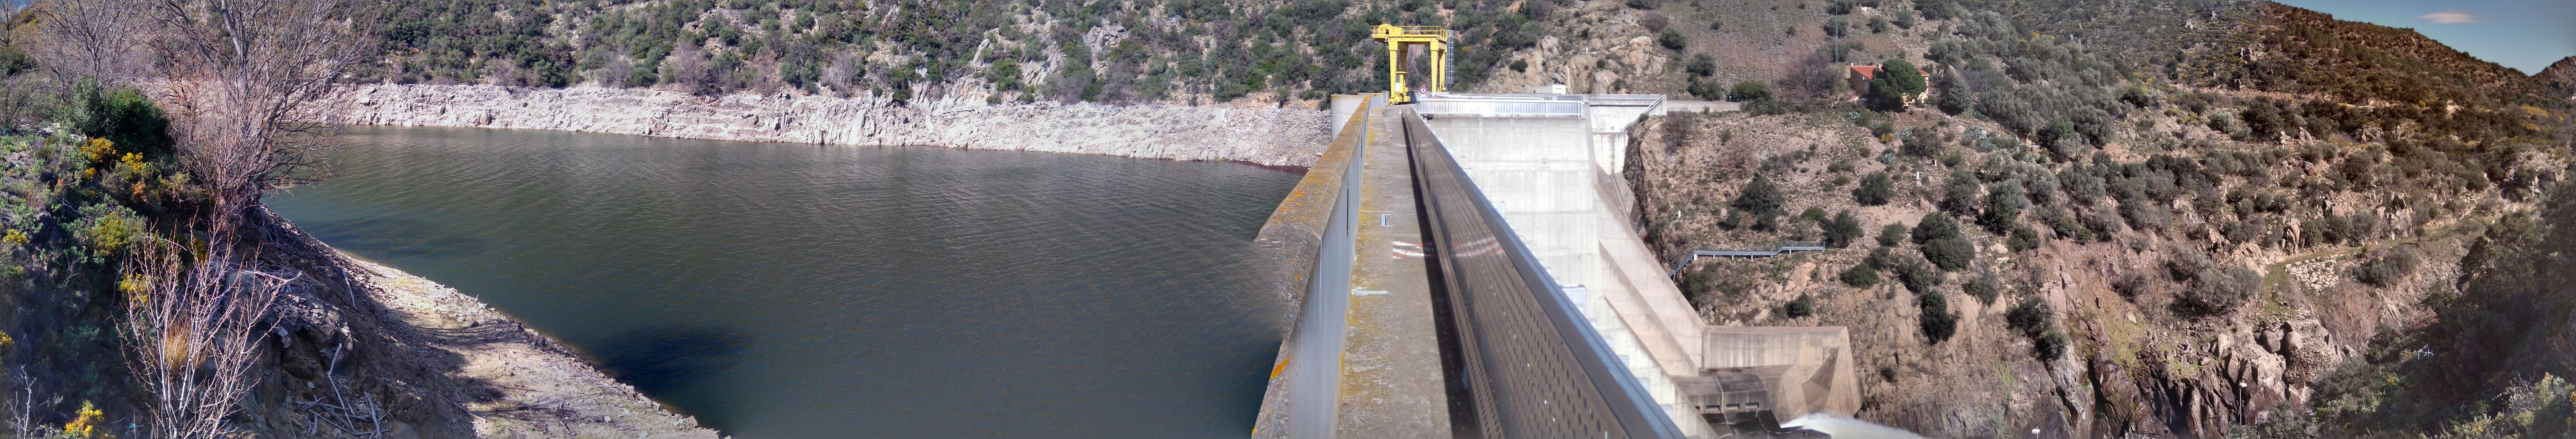
\includegraphics[width = 1\textwidth]{img/DSC_0126-PANO}
	\caption{Vinça Dam (2016-02-10)}
\end{figure}
\end{frame}

%-=-=-=-=-=-=-=-=-=-=-=-=-=-=-=-=-=-=-=-=-=-=-=-=
%	FRAME: context 
%-=-=-=-=-=-=-=-=-=-=-=-=-=-=-=-=-=-=-=-=-=-=-=-=

\section{Context}

%-=-=-=-=-=-=-=-=-=-=-=-=-=-=-=-=-=-=-=-=-=-=-=-=
%	FRAME: Map
%-=-=-=-=-=-=-=-=-=-=-=-=-=-=-=-=-=-=-=-=-=-=-=-=

\begin{frame}[c]{Map of France}
\vspace{-2em}
\begin{figure}
	\centering
	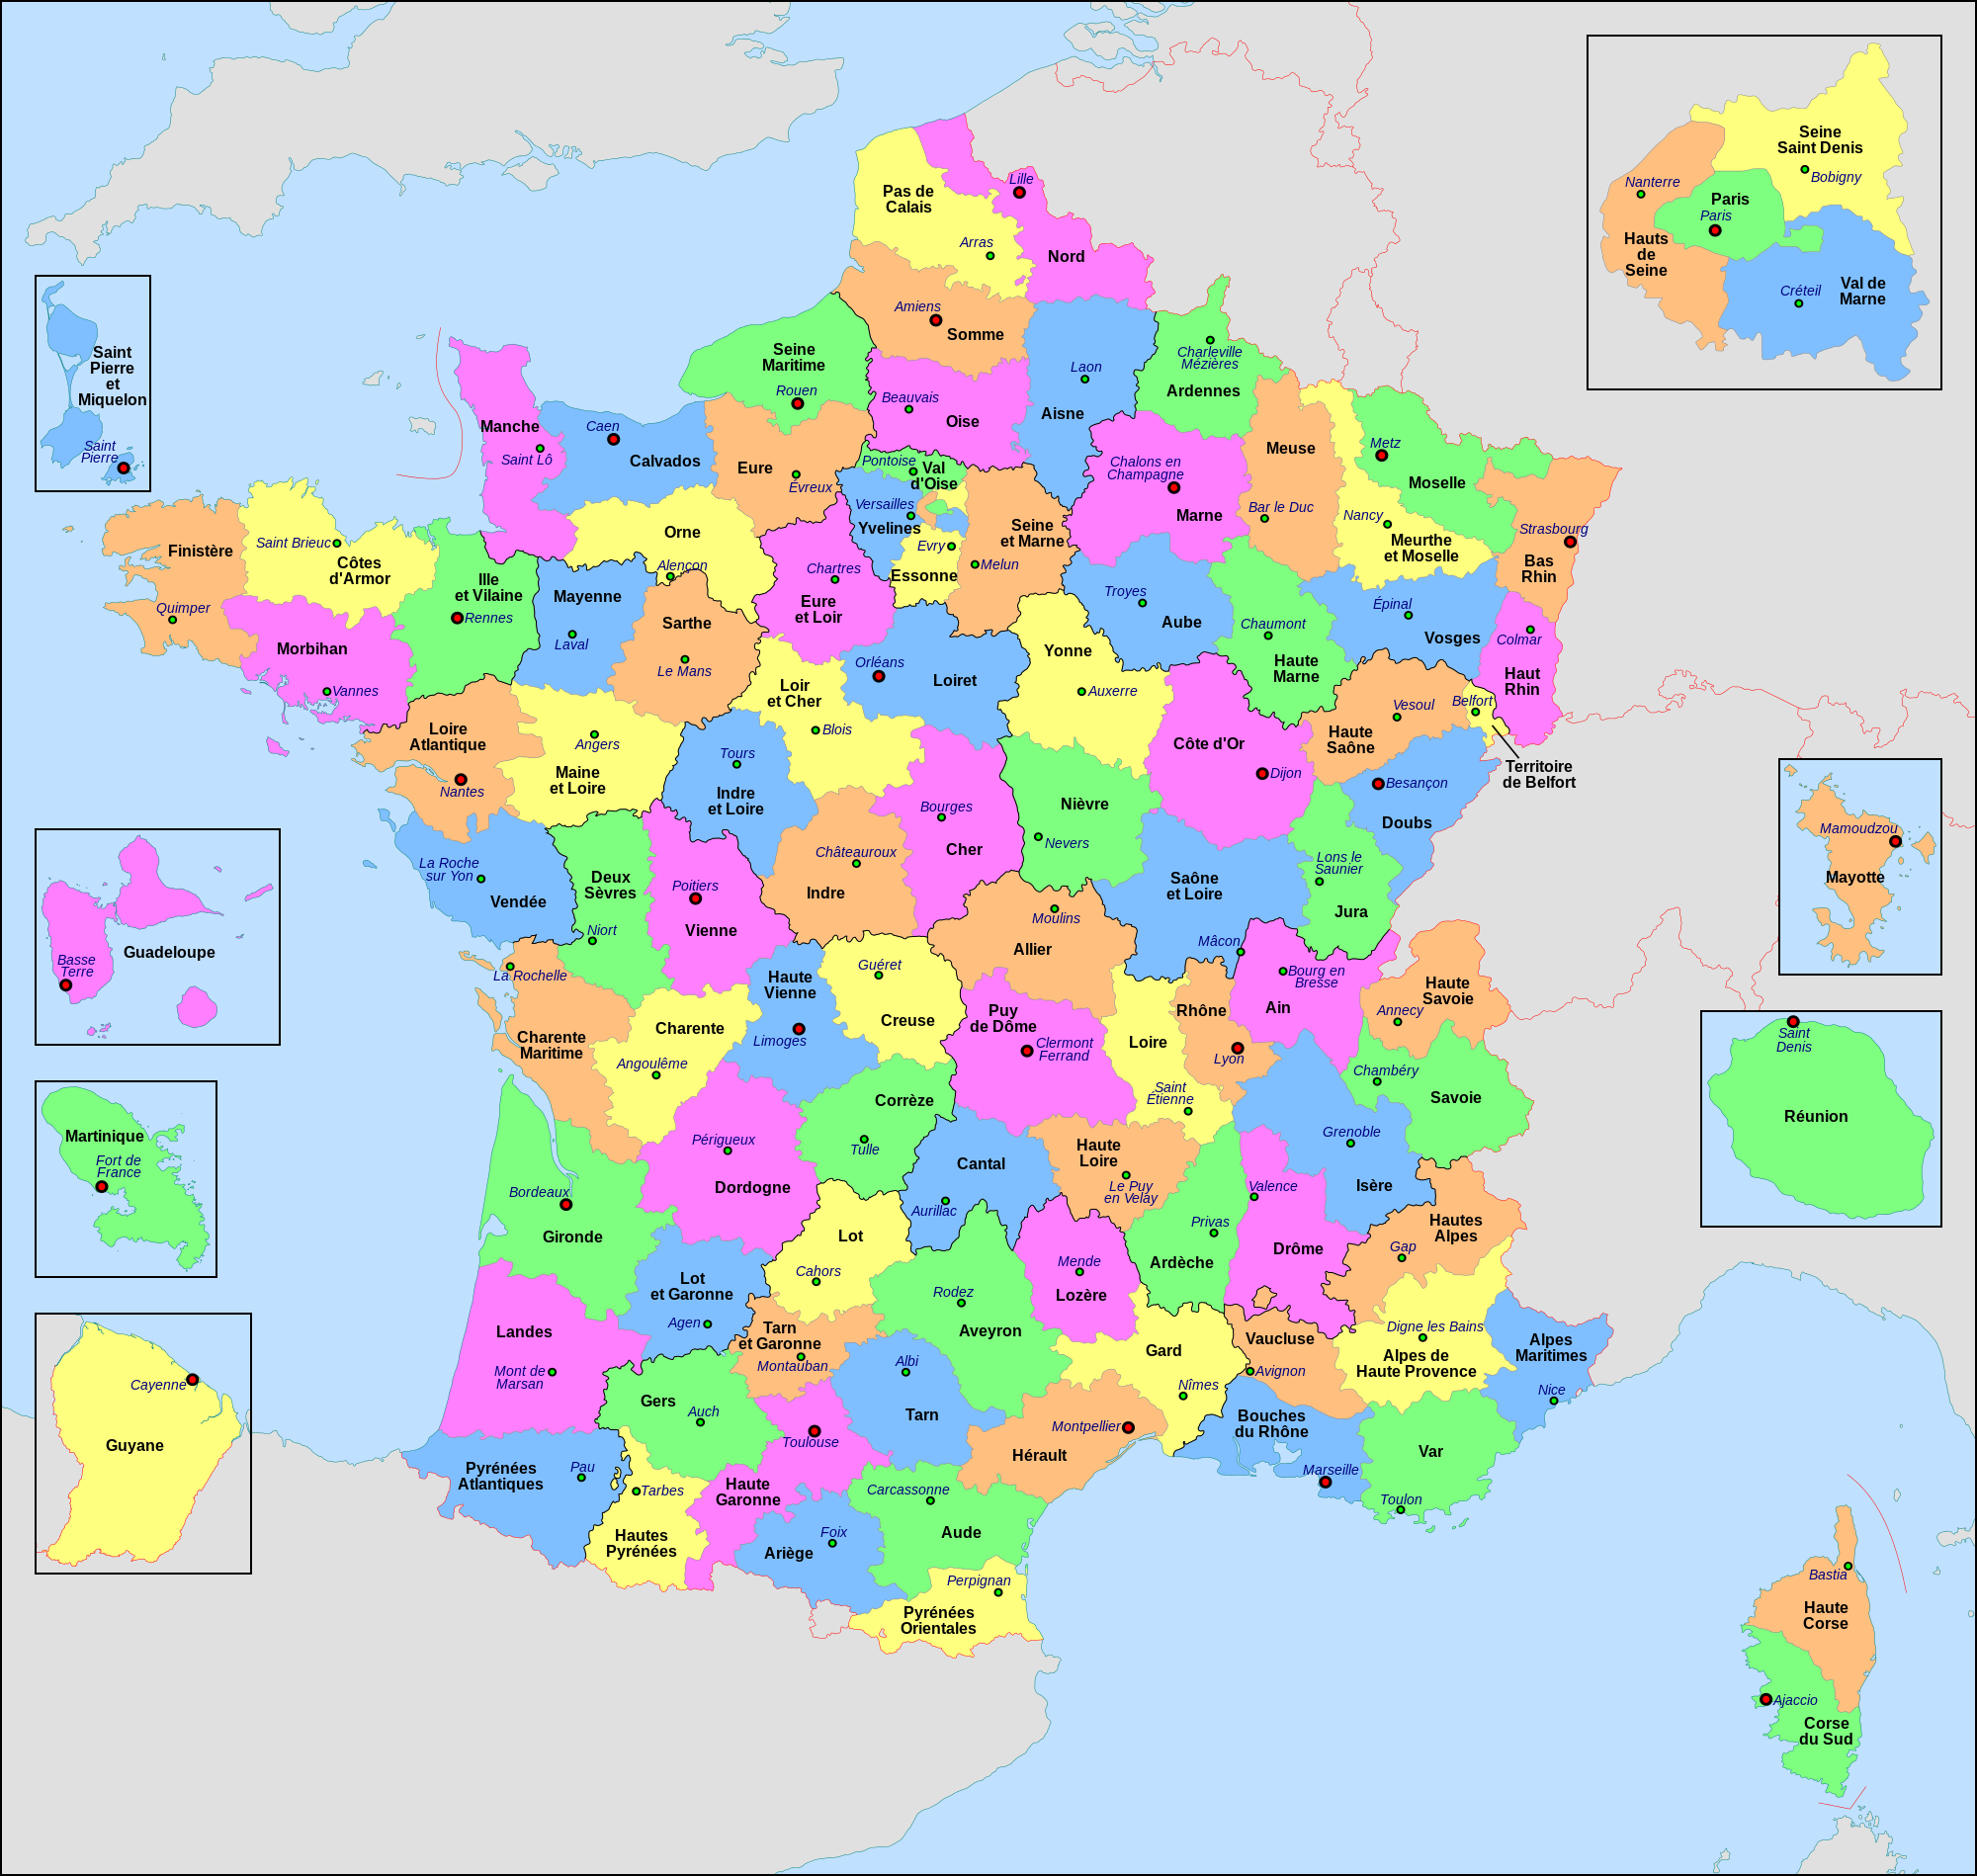
\includegraphics[width = 8cm]{img/map_france}
\end{figure}
\end{frame}

%-=-=-=-=-=-=-=-=-=-=-=-=-=-=-=-=-=-=-=-=-=-=-=-=
%	FRAME: SURFACE WATER IN PO
%-=-=-=-=-=-=-=-=-=-=-=-=-=-=-=-=-=-=-=-=-=-=-=-=

\begin{frame}[c]{Surface water in Eastern Pyrenees region}
\vspace{-4em}
\begin{figure}
	\hspace*{-0.6cm}
	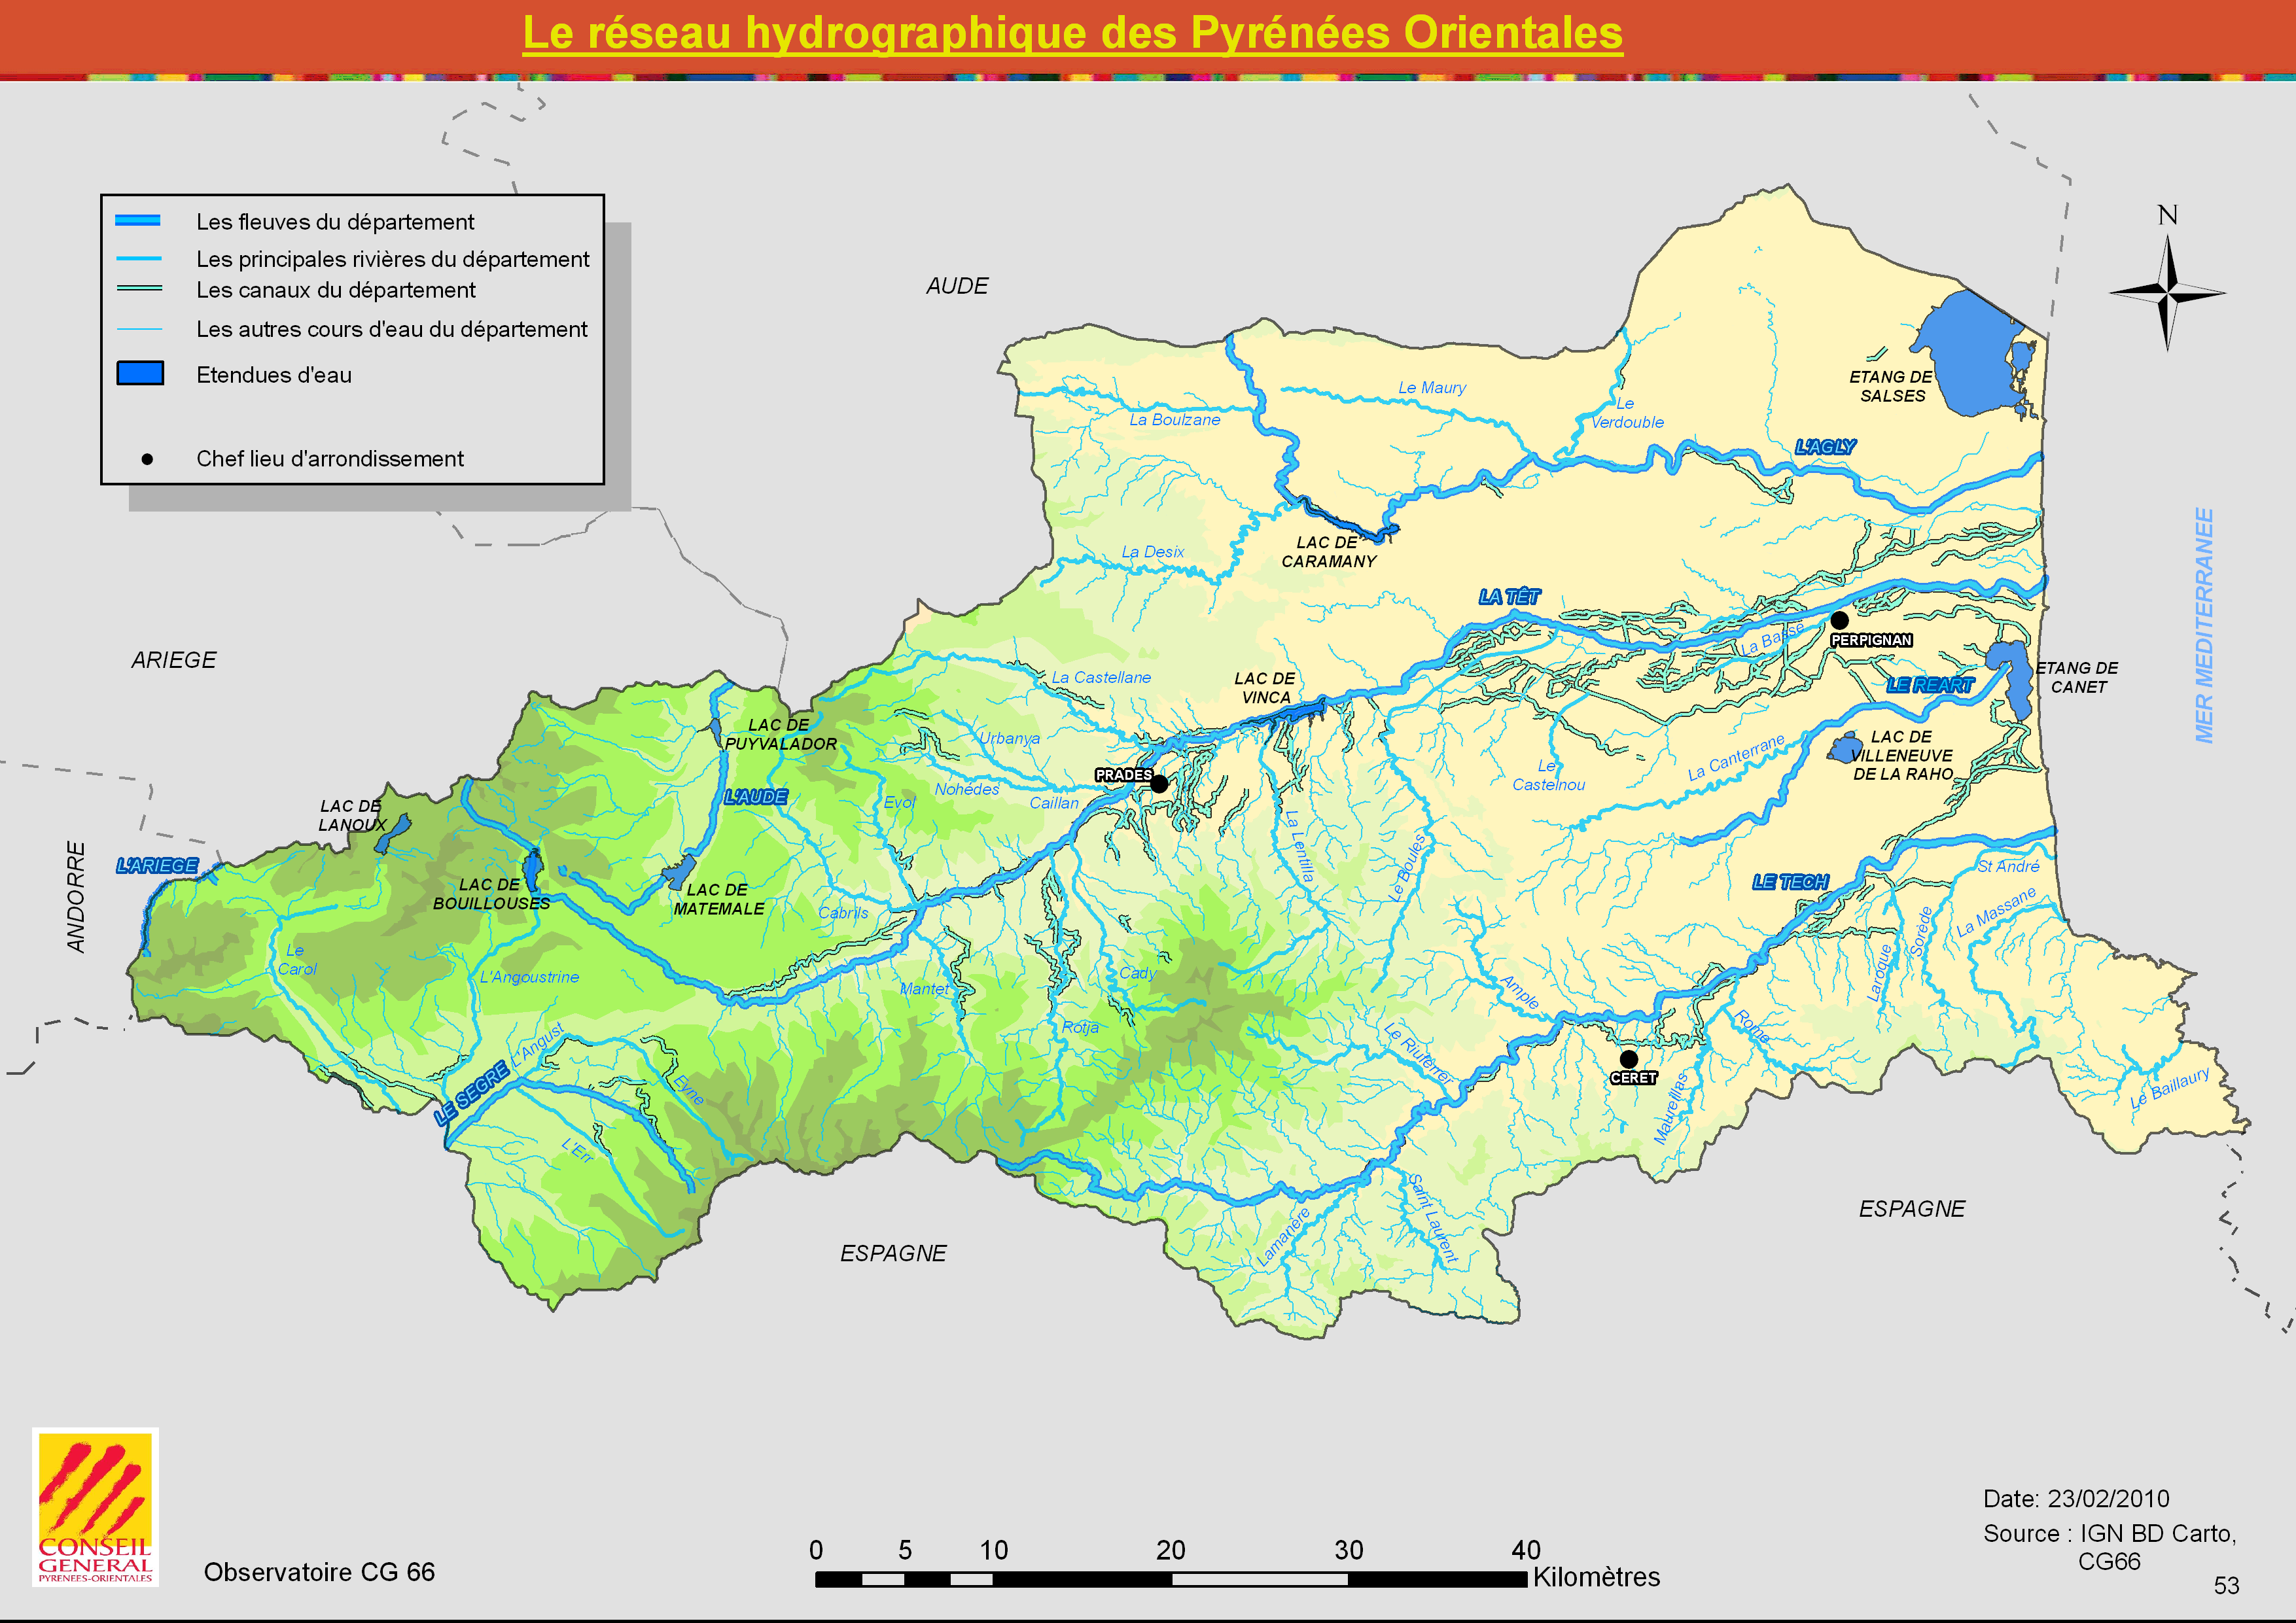
\includegraphics[width = 1.1\textwidth]{img/canaux_po}
\end{figure}
\end{frame}

%-=-=-=-=-=-=-=-=-=-=-=-=-=-=-=-=-=-=-=-=-=-=-=-=
%	FRAME: 
%-=-=-=-=-=-=-=-=-=-=-=-=-=-=-=-=-=-=-=-=-=-=-=-=

\begin{frame}[c]{Context}
\vspace{-2em}
\begin{itemize}
	\item Study focused on the Têt basin between Vinça  and Perpignan
	\item Mediterranean climate
	\item Irrigation history
\end{itemize}
\begin{figure}
	
	\subfigure[]{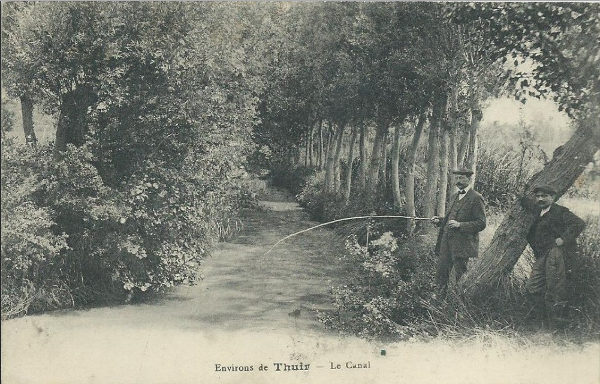
\includegraphics[width = 5cm]{img/canalThuir}}
	\subfigure[]{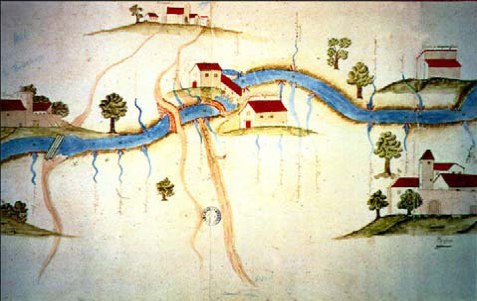
\includegraphics[width = 5cm]{img/canal_thuyr}}
\end{figure}

\end{frame}

%-=-=-=-=-=-=-=-=-=-=-=-=-=-=-=-=-=-=-=-=-=-=-=-=
%	FRAME: IRRIGATED AGRICULTURAL LAND IN FRANCCE
%-=-=-=-=-=-=-=-=-=-=-=-=-=-=-=-=-=-=-=-=-=-=-=-=

\begin{frame}[c]{Irrigated agricultural land in France}
\vspace{-2em}
\begin{figure}
	\centering
	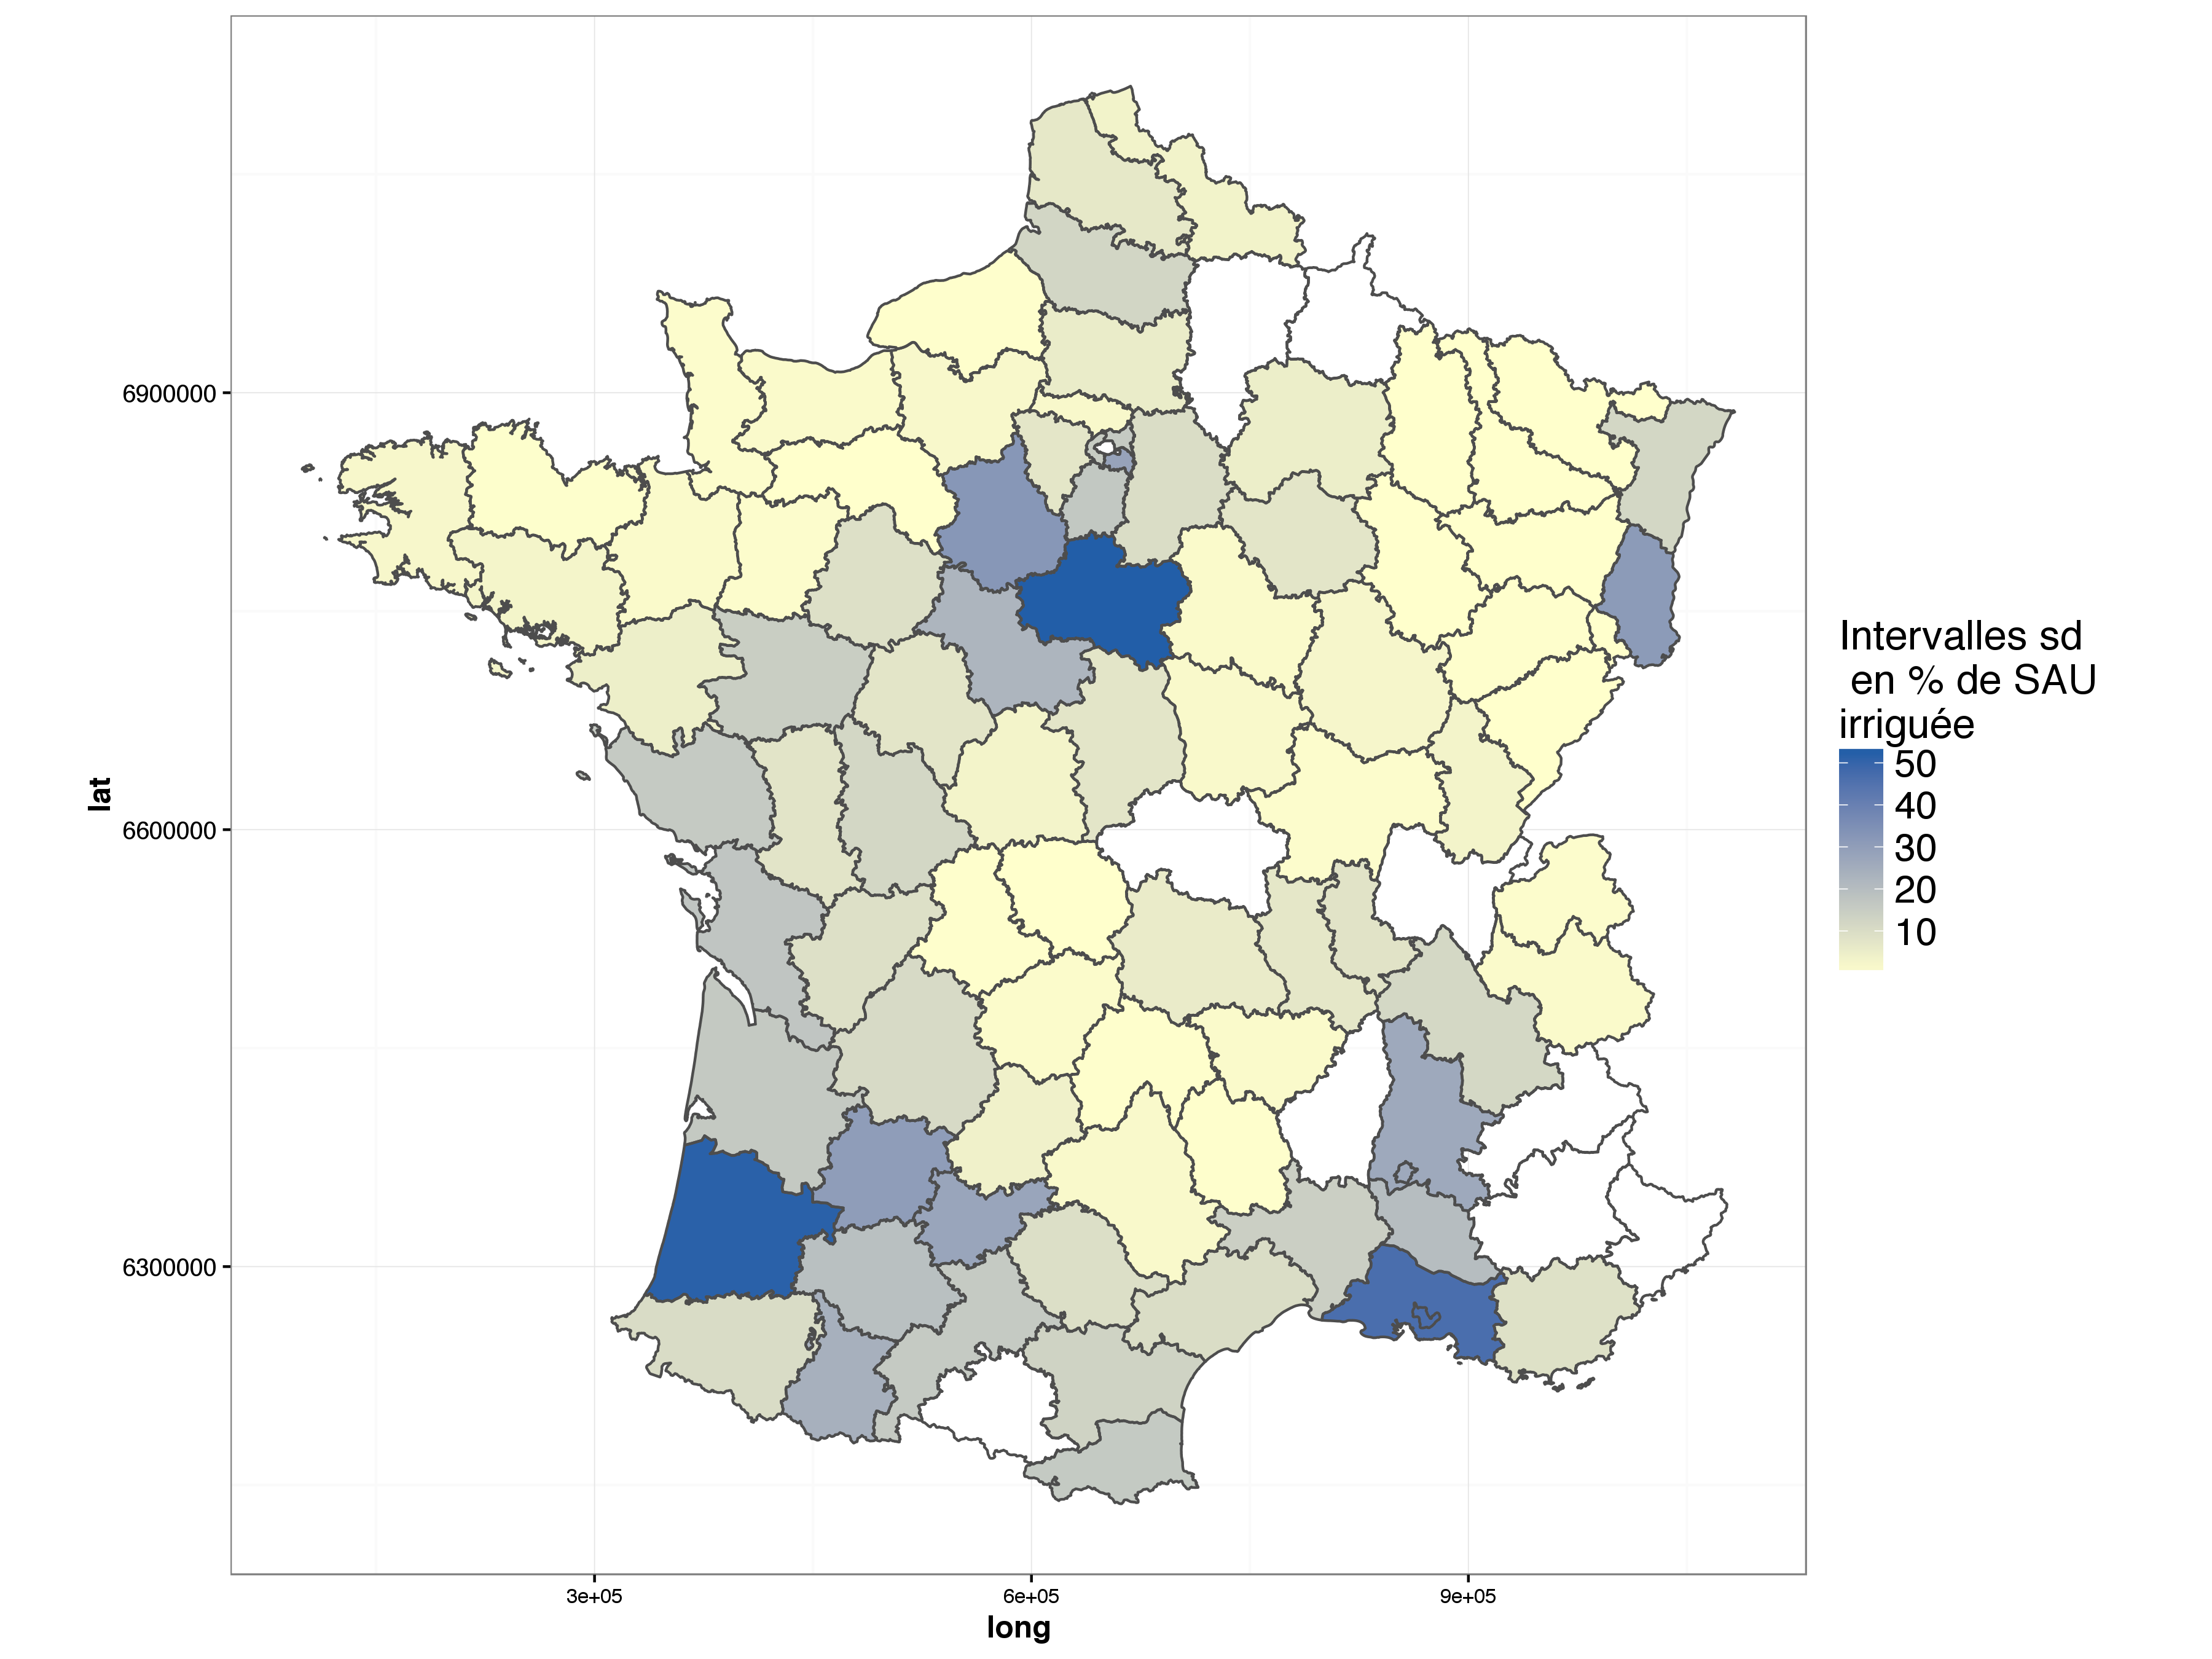
\includegraphics[width = 0.8\textwidth]{img/SAU}
\end{figure}
\small{Source : GEOFLA, Agreste -- Disar, RA 2010}

\end{frame}

%-=-=-=-=-=-=-=-=-=-=-=-=-=-=-=-=-=-=-=-=-=-=-=-=
%	FRAME: INSTEAD OF COLLECTIVE IRRIGATION IN FRANCE
%-=-=-=-=-=-=-=-=-=-=-=-=-=-=-=-=-=-=-=-=-=-=-=-=

\begin{frame}[c]{Collective irrigation}
\vspace{-2em}
\begin{figure}
	\centering
	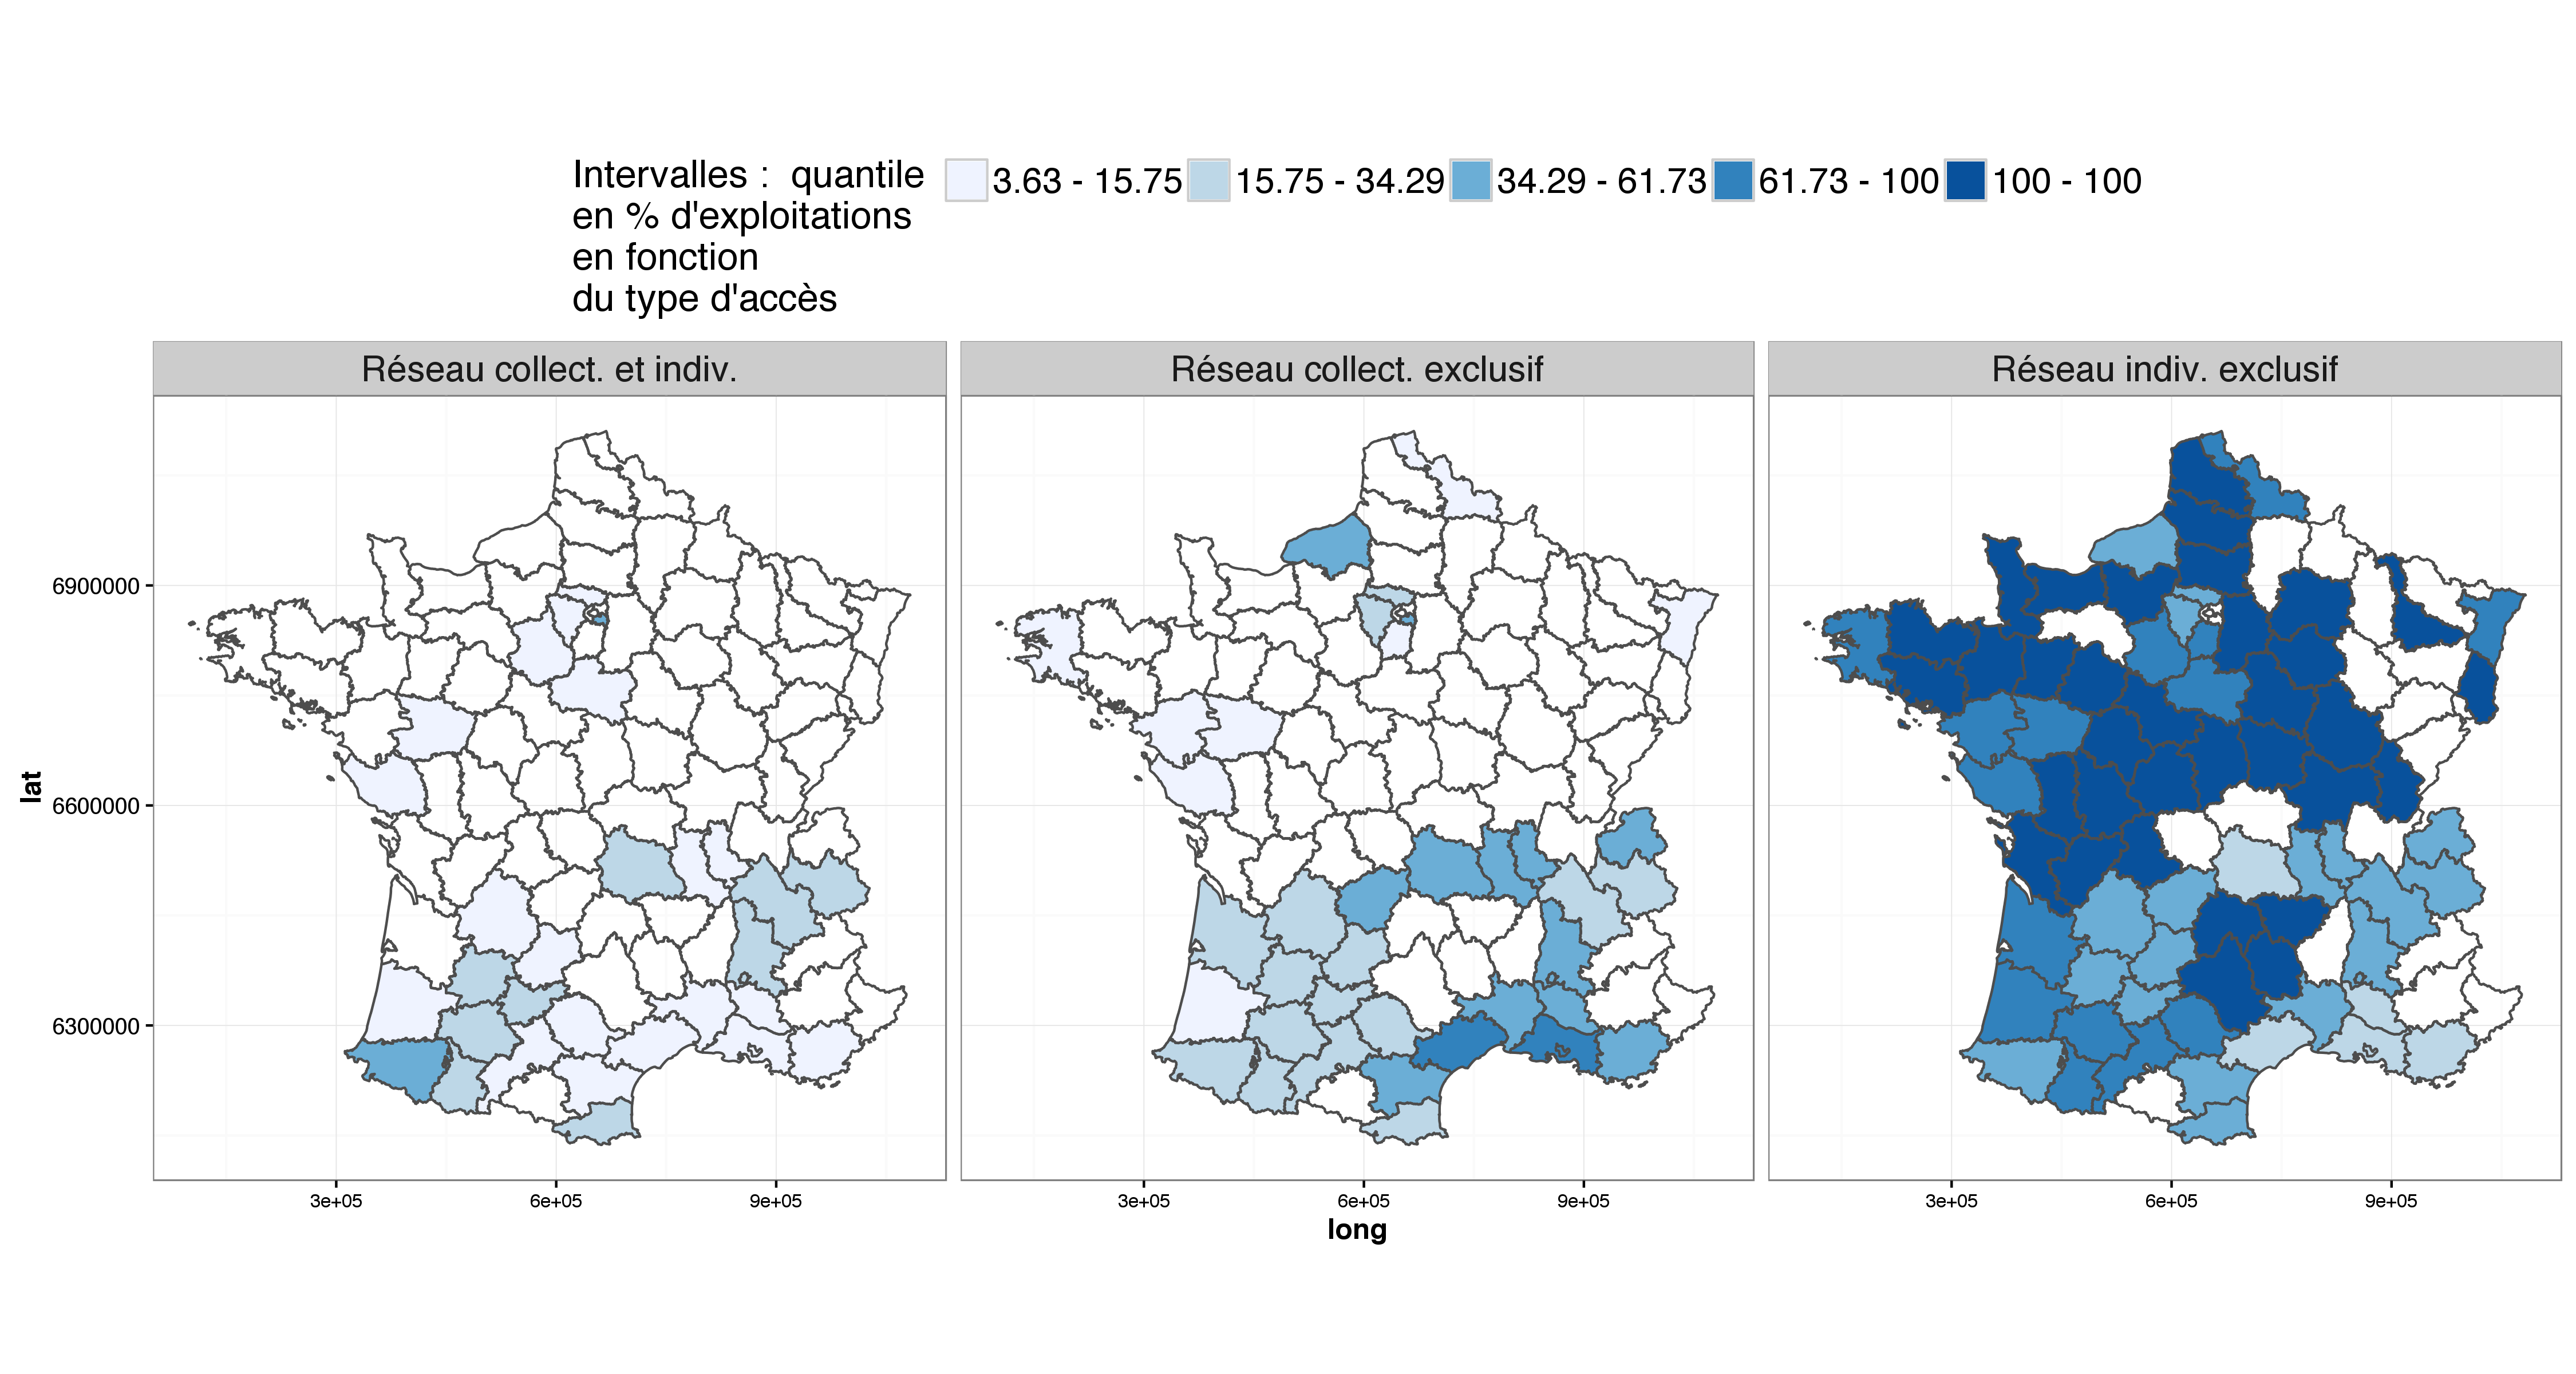
\includegraphics[width = 1\textwidth]{img/nb_irrigant2}
\end{figure}
\small{Source : GEOFLA, Agreste -- Disar, RA 2010}

\end{frame}

%-=-=-=-=-=-=-=-=-=-=-=-=-=-=-=-=-=-=-=-=-=-=-=-=
%	FRAME: ASA
%-=-=-=-=-=-=-=-=-=-=-=-=-=-=-=-=-=-=-=-=-=-=-=-=

\begin{frame}[c]{Authorized Syndicated Association}
An Authorized Syndicated Association is a legal entity that brings together owners of adjacent properties to collectivize and coordinate the development, use, and maintenance of irrigation canals.
\begin{figure}
	\centering
	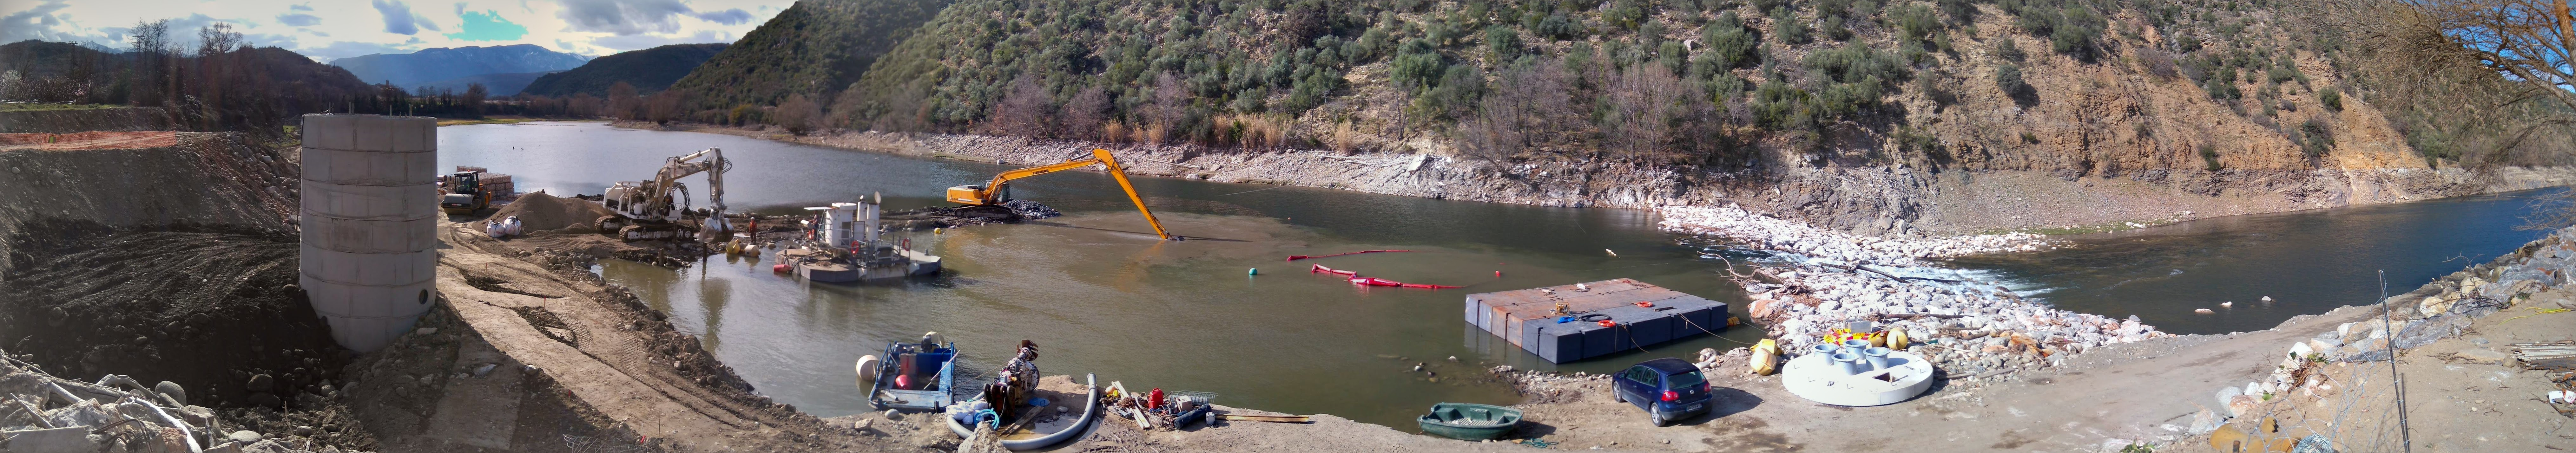
\includegraphics[width = 1\textwidth]{img/DSC_0196-PANO}
	\caption{Development work carried out by ASA of Vinca (2016-02-12)}
\end{figure}
\end{frame}

%-=-=-=-=-=-=-=-=-=-=-=-=-=-=-=-=-=-=-=-=-=-=-=-=
%	FRAME: ASA 1
%-=-=-=-=-=-=-=-=-=-=-=-=-=-=-=-=-=-=-=-=-=-=-=-=

\begin{frame}[c]{Authorized Syndicated Associations (France)}
\vspace{-3em}
\begin{figure}
	\centering
	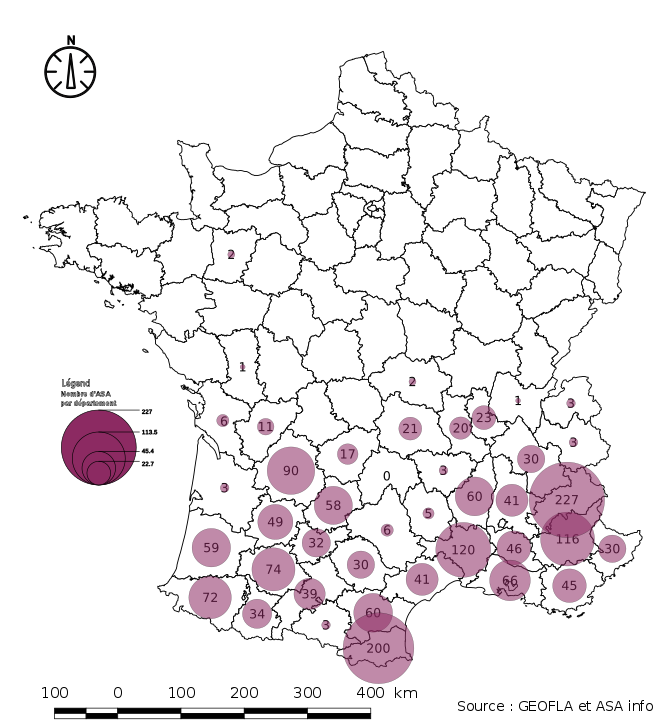
\includegraphics[width = 0.65\textwidth]{img/nbASA_dep}
\end{figure}
\end{frame}


%-=-=-=-=-=-=-=-=-=-=-=-=-=-=-=-=-=-=-=-=-=-=-=-=
%	THE HYDRAULIC SOCIETY IN THE EASTERN PYRENNES
%-=-=-=-=-=-=-=-=-=-=-=-=-=-=-=-=-=-=-=-=-=-=-=-=

\section{Hydraulic society in the Eastern Pyrenees?}


%-=-=-=-=-=-=-=-=-=-=-=-=-=-=-=-=-=-=-=-=-=-=-=-=
%	FRAME:
%-=-=-=-=-=-=-=-=-=-=-=-=-=-=-=-=-=-=-=-=-=-=-=-=

\begin{frame}[c]{Wittfogel ? }
\begin{itemize}
	\item Wittfogel’s dialectical insights into the relations between the control of water and the control of people help explain the effects of the Vinça dam, which we argue was built partly as a means of gaining territorial presence in a region historically resistant to the control of the French state.
	\item We suggest that the dam has had the effect of weakening local social relations that were sustained by the need to deal with hydrological uncertainty.
\end{itemize}
\end{frame}

%-=-=-=-=-=-=-=-=-=-=-=-=-=-=-=-=-=-=-=-=-=-=-=-=
%	FRAME:
%-=-=-=-=-=-=-=-=-=-=-=-=-=-=-=-=-=-=-=-=-=-=-=-=

\begin{frame}[c]{Water control and the French state}
\vspace{-2em}
A Long history!

\begin{itemize}
	\item Rosenthal (1988) shows how this process accelerated after the Revolution for irrigation and drainage
	\item However, the Eastern Pyrenees region avoided or resisted these encroachments until very late
	\item Jaubert de Passa (1820)
	\begin{itemize}
		\item Local irrigation traditions
		\item Isolation from French state
	\end{itemize}
\end{itemize}
\begin{figure}
	\centering
	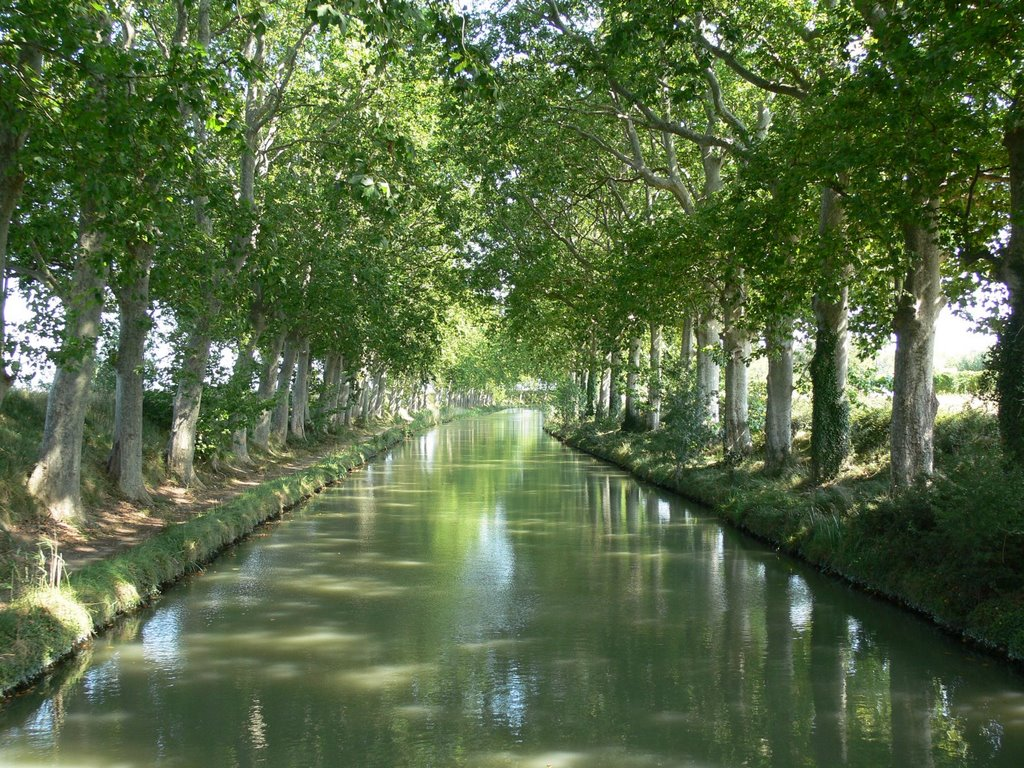
\includegraphics[width = 0.65\textwidth]{img/canal_midi}
\end{figure}
\end{frame}

%-=-=-=-=-=-=-=-=-=-=-=-=-=-=-=-=-=-=-=-=-=-=-=-=
%	FRAME:
%-=-=-=-=-=-=-=-=-=-=-=-=-=-=-=-=-=-=-=-=-=-=-=-=

\begin{frame}[c]{The Vinça Dam }
\begin{itemize}
	\item First proposal to build a dam at Vinça to control floods and facilitate irrigation was put forward early 20th century
	\item Leon Jean Grégory (1909-1982): “Surface water for irrigation; groundwater for drinking”
	\item Preliminary studies found a deficit between availability of water and the needs of farmers.
\end{itemize}
\begin{figure}
	\centering
	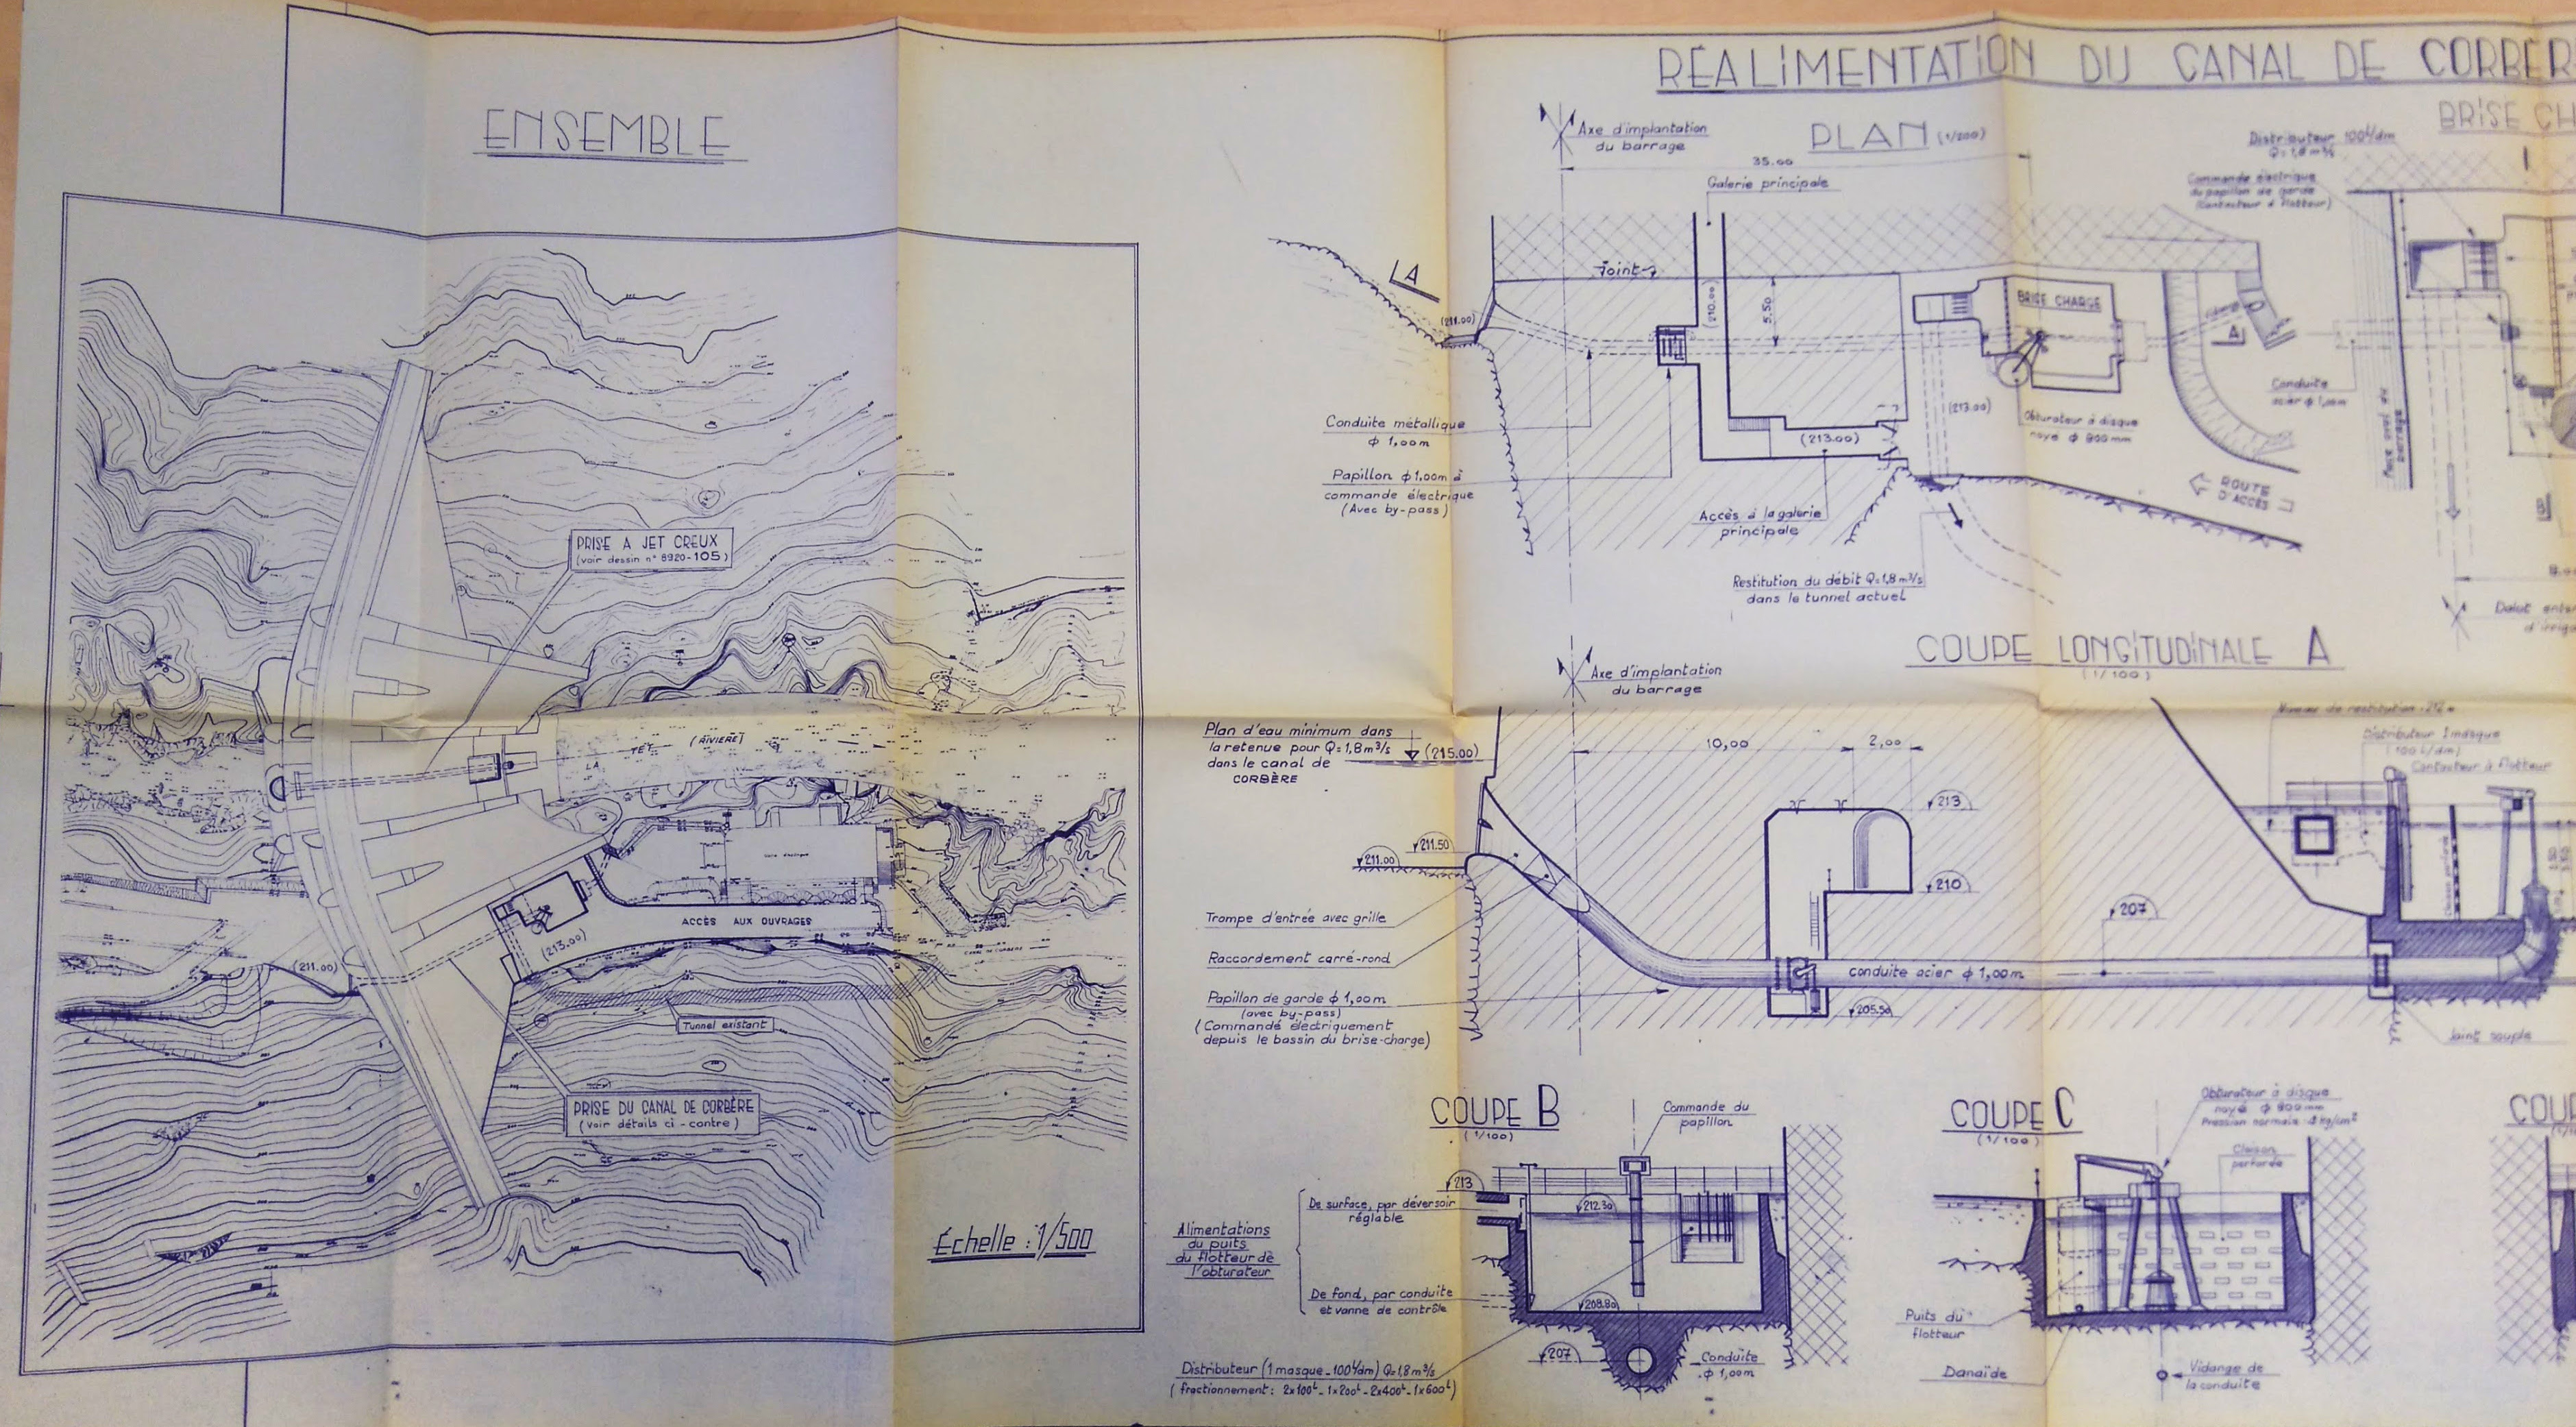
\includegraphics[width = 0.7\textwidth]{img/plan-barrage}
	 \caption{Dam plan (Archive des Pyrénées Orientales 1388w12)}
\end{figure}

\end{frame}


%-=-=-=-=-=-=-=-=-=-=-=-=-=-=-=-=-=-=-=-=-=-=-=-=
%	FRAME: DAM JUSTIFICATION
%-=-=-=-=-=-=-=-=-=-=-=-=-=-=-=-=-=-=-=-=-=-=-=-=

\begin{frame}[c]{Justifying the Vinça Dam (producing scarcity) }

\begin{quote}
	"To illustrate the imbalance between needs and resources, we will quote two figures, one of $14 m^3$ / second,  corresponding to the water rights of the ASAs,  and $5.5$ , $2.4$, and $4 m^3$ / second, corresponding to the average flows at Vinça in July, August and September, given the release of water made from the dam at Bouillouse, it being understood that the actual flow rates during drought significantly falls below these values."
\end{quote}
D.U.P. (Declaration of Public Utility) for the Vinça Dam project, August 27, 1970
\end{frame}

%-=-=-=-=-=-=-=-=-=-=-=-=-=-=-=-=-=-=-=-=-=-=-=-=
%	FRAME:HOSTILITY ?
%-=-=-=-=-=-=-=-=-=-=-=-=-=-=-=-=-=-=-=-=-=-=-=-=

\begin{frame}[c]{Hostility or indifference to the dam}
\vspace{-2em}
Public inquiry revealed that contrary to expectations, the farmers did not particularly want a dam

\begin{itemize}
	\item Impact on farmland
	\item Money better applied to improvement of canals
	\item Preference for small upland dams
\end{itemize}
\begin{figure}
	\centering
	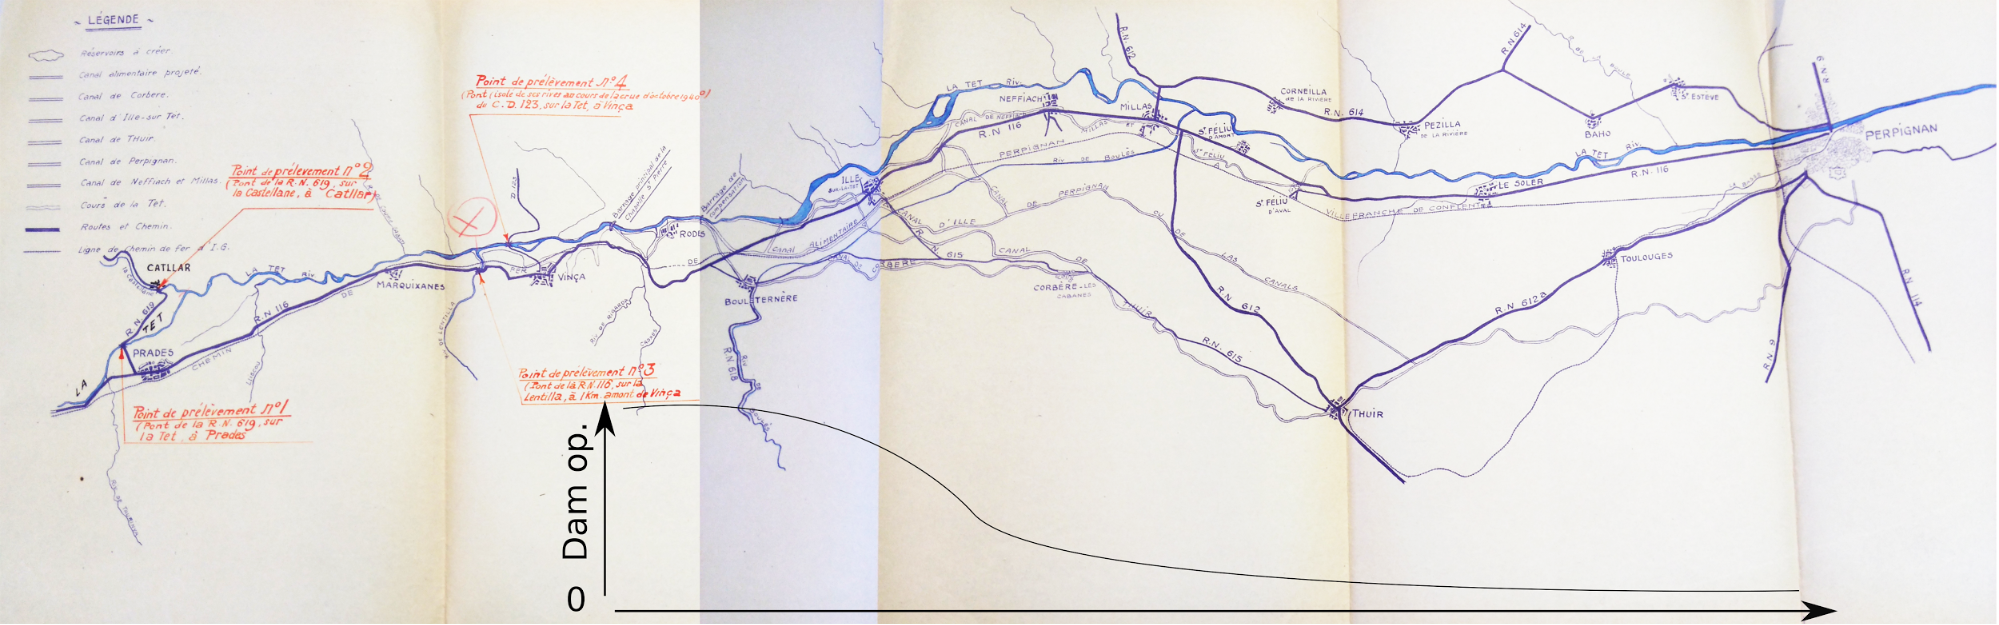
\includegraphics[width = \textwidth]{img/epiphenomene}
	 \caption{hostility towards the dam}
\end{figure}
\end{frame}

%-=-=-=-=-=-=-=-=-=-=-=-=-=-=-=-=-=-=-=-=-=-=-=-=
%	FRAME: DEATH
%-=-=-=-=-=-=-=-=-=-=-=-=-=-=-=-=-=-=-=-=-=-=-=-=

\section{Death by certainty}

%-=-=-=-=-=-=-=-=-=-=-=-=-=-=-=-=-=-=-=-=-=-=-=-=
%	FRAME: DAM HISTORY
%-=-=-=-=-=-=-=-=-=-=-=-=-=-=-=-=-=-=-=-=-=-=-=-=

\begin{frame}[c]{The dam history}
\vspace{-0.5cm}

\startchronology[startyear=1900, stopyear=2000]
\chronoevent[markdepth=60pt]{1910}{first study}%order - furthest out first
\chronoevent{1920}{\cBlue{flood}}
\chronoevent{1940}{\cBlue{flood}}
\chronoperiode{1953}{1965}{second study}
\chronoevent[markdepth=50pt, textwidth=2cm]{1954}{first union of ASAs}
\chronoevent[markdepth=12pt, textwidth=2.5cm]{1976}{\cRed{dam impoundment}}
\chronoevent[markdepth=60pt, textwidth=2.5cm]{1989}{first Corbère pumping stations}
\stopchronology

\vspace{-1em}
Dam goals
\begin{itemize}
	\item pool of water for agriculture,
	\item reduce flood peaks ,
	\item drinking water storage.
\end{itemize}

\end{frame}

%-=-=-=-=-=-=-=-=-=-=-=-=-=-=-=-=-=-=-=-=-=-=-=-=
%	FRAME: Death ?
%-=-=-=-=-=-=-=-=-=-=-=-=-=-=-=-=-=-=-=-=-=-=-=-=

\begin{frame}[c]{Death by certainty}
We argue that the dam has had the effect of transferring expertise and social power from local to central authority, but not just in a direct way:

\begin{itemize}
	\item The state controls the dam (through the Department)
	\item But the most important means by which local control has been reduced is indirectly through the state’s (Agence de l’eau) promotion of pressurized irrigation, which the dam makes possible 
	\item Gravity irrigation structures a set of social relations that are different from those structured by pressurized irrigation
	\item Pressurized irrigation is more efficient and less arduous, but weakens the social tissues that are put in place and maintained by the condition of hydrological uncertainty
\end{itemize}
\end{frame}

%-=-=-=-=-=-=-=-=-=-=-=-=-=-=-=-=-=-=-=-=-=-=-=-=
%	FRAME: Conclusion
%-=-=-=-=-=-=-=-=-=-=-=-=-=-=-=-=-=-=-=-=-=-=-=-=

\section{Conclusions}


%-=-=-=-=-=-=-=-=-=-=-=-=-=-=-=-=-=-=-=-=-=-=-=-=
%	FRAME: Death ?
%-=-=-=-=-=-=-=-=-=-=-=-=-=-=-=-=-=-=-=-=-=-=-=-=

\begin{frame}[c]{Conclusions and next steps…}
\begin{itemize}
	\item The scarcity argument used in 1970 to build the dam and produce certainty for agricultural production is now used to support reductions in the use of water by farmers through promotion of pressurized irrigation.
	\item This threatens traditional ASAs, which are wary of the state’s encroachment on their water rights.
	\item Unintended implications for groundwater recharge.
	\item We hypothesize that longer-term consequences of the dam include unintended impacts on the agricultural sector.
\end{itemize}
\end{frame}



%-=-=-=-=-=-=-=-=-=-=-=-=-=-=-=-=-=-=-=-=-=-=-=-=
%	FRAME: MERCI DE VOTRE ATTENTION
%-=-=-=-=-=-=-=-=-=-=-=-=-=-=-=-=-=-=-=-=-=-=-=-=
{
\usebackgroundtemplate{
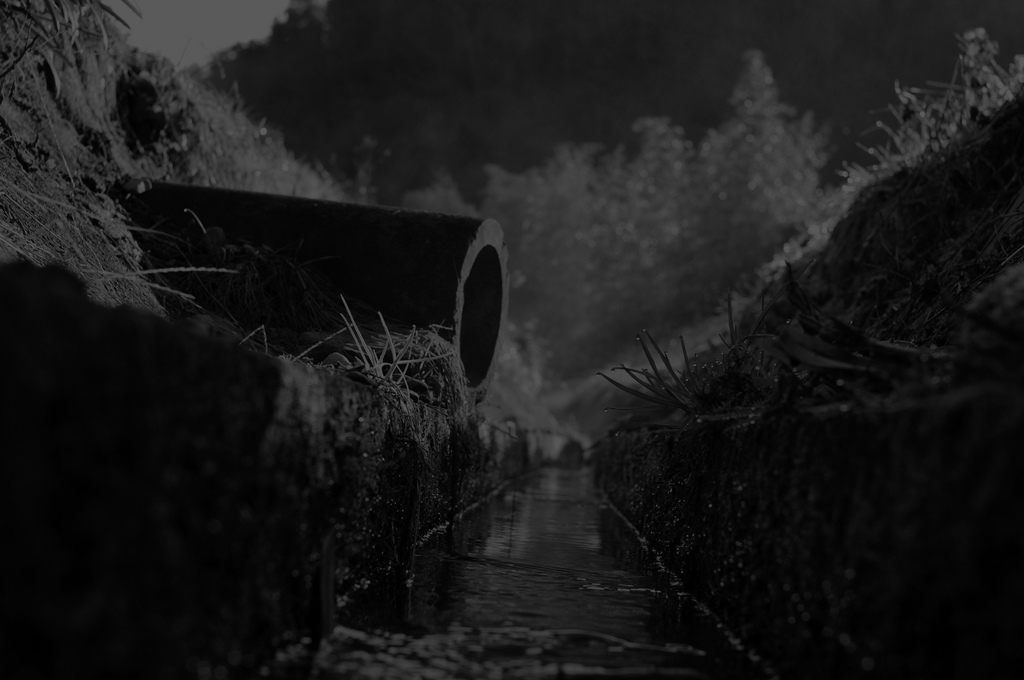
\includegraphics[width=\paperwidth]{img/fin.jpg}}%
\begin{frame}
  \vspace{-1em}  
  \begin{minipage}[t][.8\textheight]{\textwidth}
    \color{\cnGrey}{\LARGE{Thank you for your attention}}

    \vfill

  \hfill \small{Photo credit : Thomas m-louis. sur 
\includegraphics[height=0.55cm]{img/flickr_logo}}
  \end{minipage}
  \vspace{-3em}
  \centering
	You can find this presentation on github
\includegraphics[height=0.85cm]{img/github}  
  
\end{frame}
}

%-=-=-=-=-=-=-=-=-=-=-=-=-=-=-=-=-=-=-=-=-=-=-=-=
%	FRAME: ANNEXE PHOTOS
%-=-=-=-=-=-=-=-=-=-=-=-=-=-=-=-=-=-=-=-=-=-=-=-=
{
\usebackgroundtemplate{
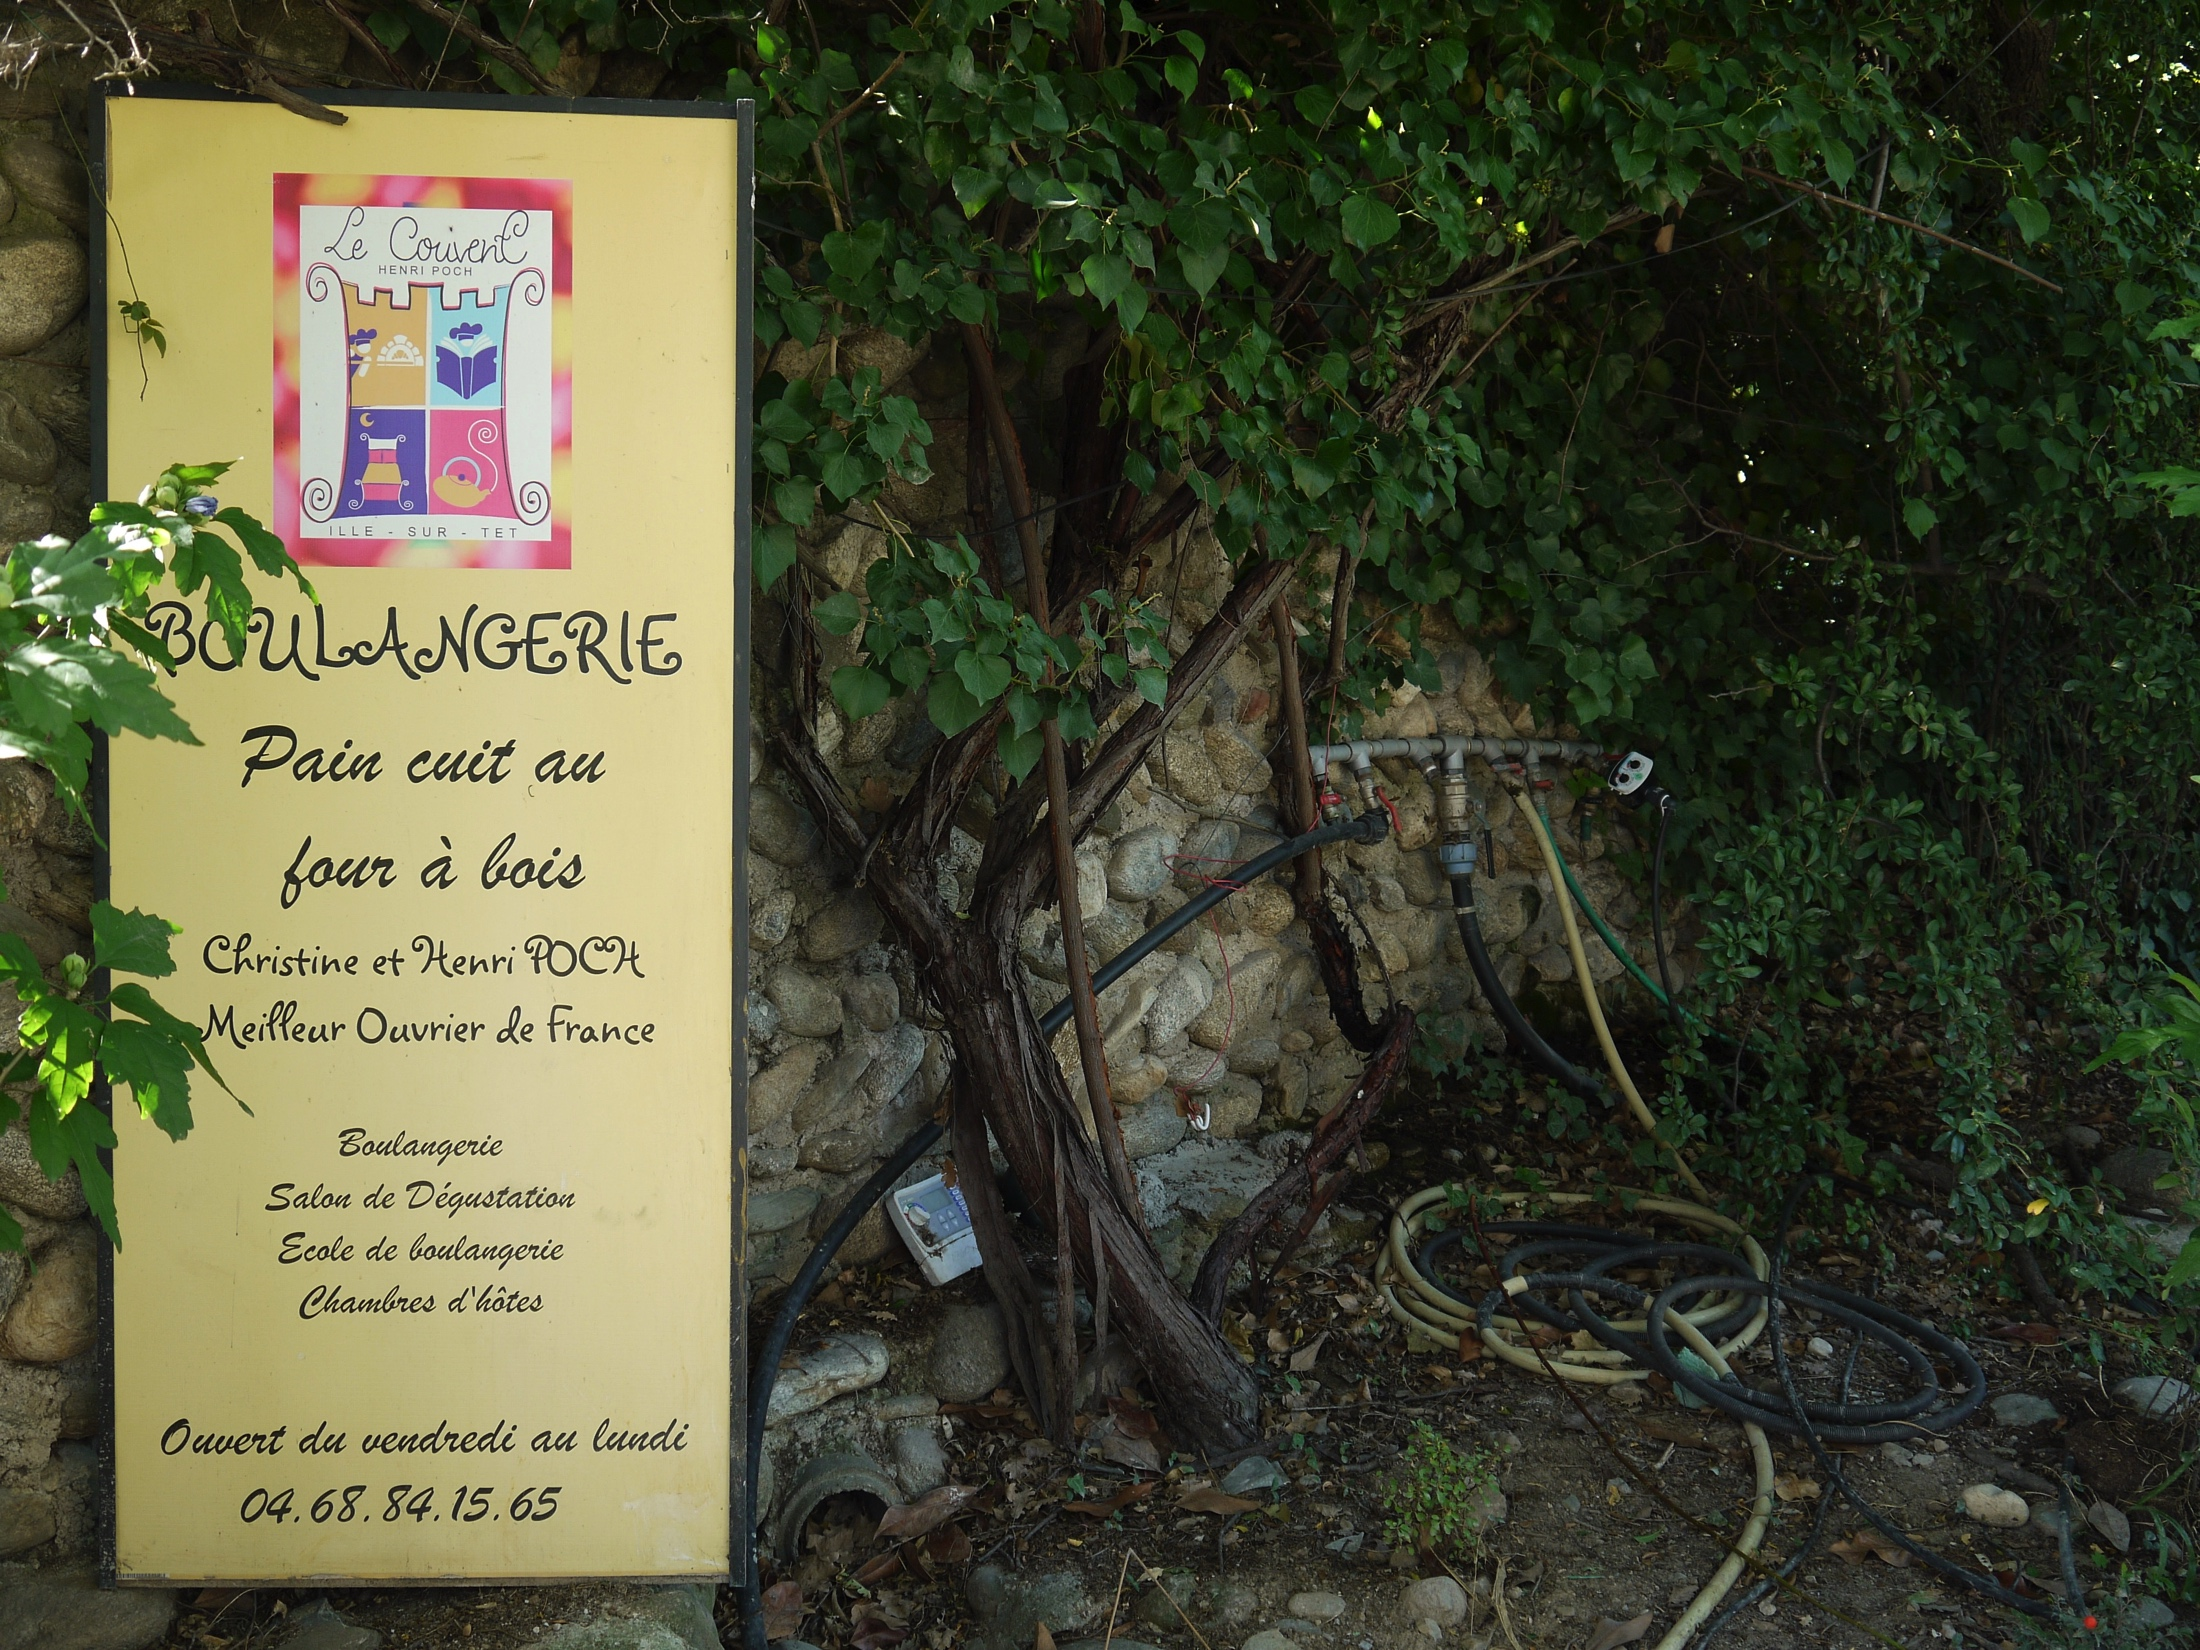
\includegraphics[width=\paperwidth]{img/annexe_boulange}}%
\begin{frame}
  \vspace{-1em}  
  \begin{minipage}[t][.8\textheight]{\textwidth}
    \color{\cnGrey}{\LARGE{~}}

    \vfill

  \hfill \small{Photo credit : James Linton}
  \end{minipage}
  
\end{frame}
}

%-=-=-=-=-=-=-=-=-=-=-=-=-=-=-=-=-=-=-=-=-=-=-=-=
{
\usebackgroundtemplate{
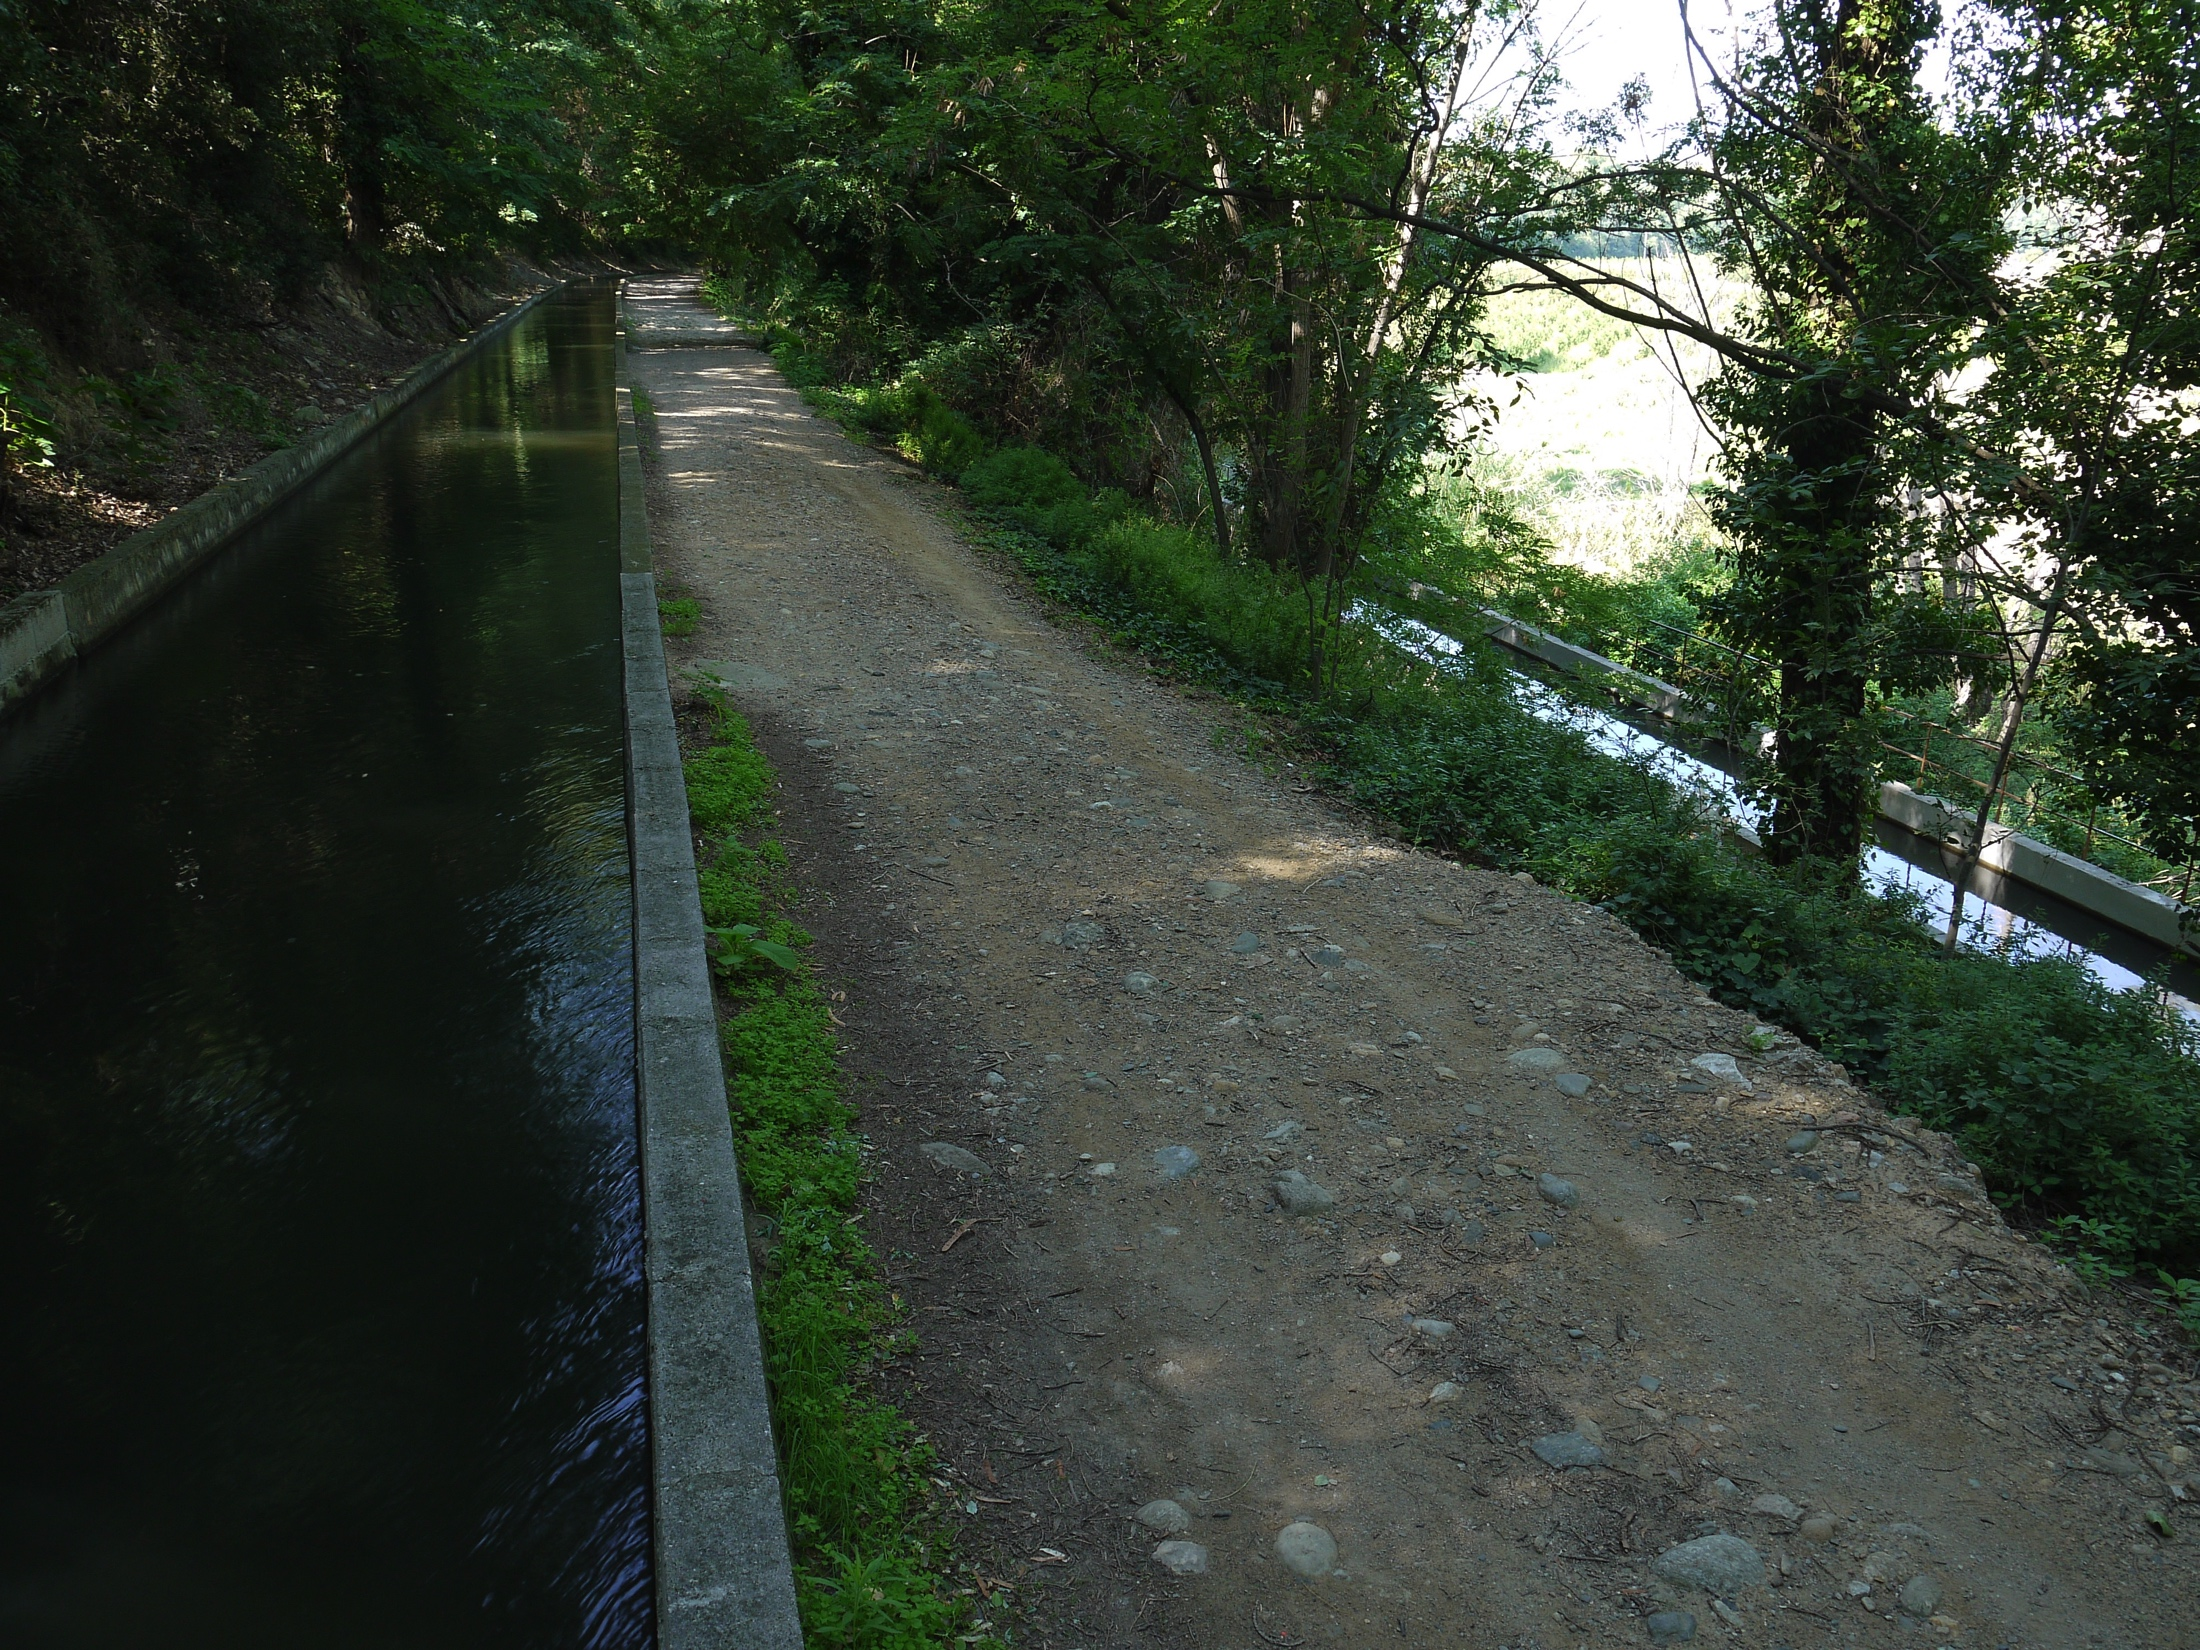
\includegraphics[width=\paperwidth]{img/annexe_canal1}}%
\begin{frame}
  \vspace{-1em}  
  \begin{minipage}[t][.8\textheight]{\textwidth}
    \color{\cnGrey}{\LARGE{~}}

    \vfill

  \hfill \small{Photo credit : James Linton}
  \end{minipage}
  
\end{frame}
}

%-=-=-=-=-=-=-=-=-=-=-=-=-=-=-=-=-=-=-=-=-=-=-=-=
{
\usebackgroundtemplate{
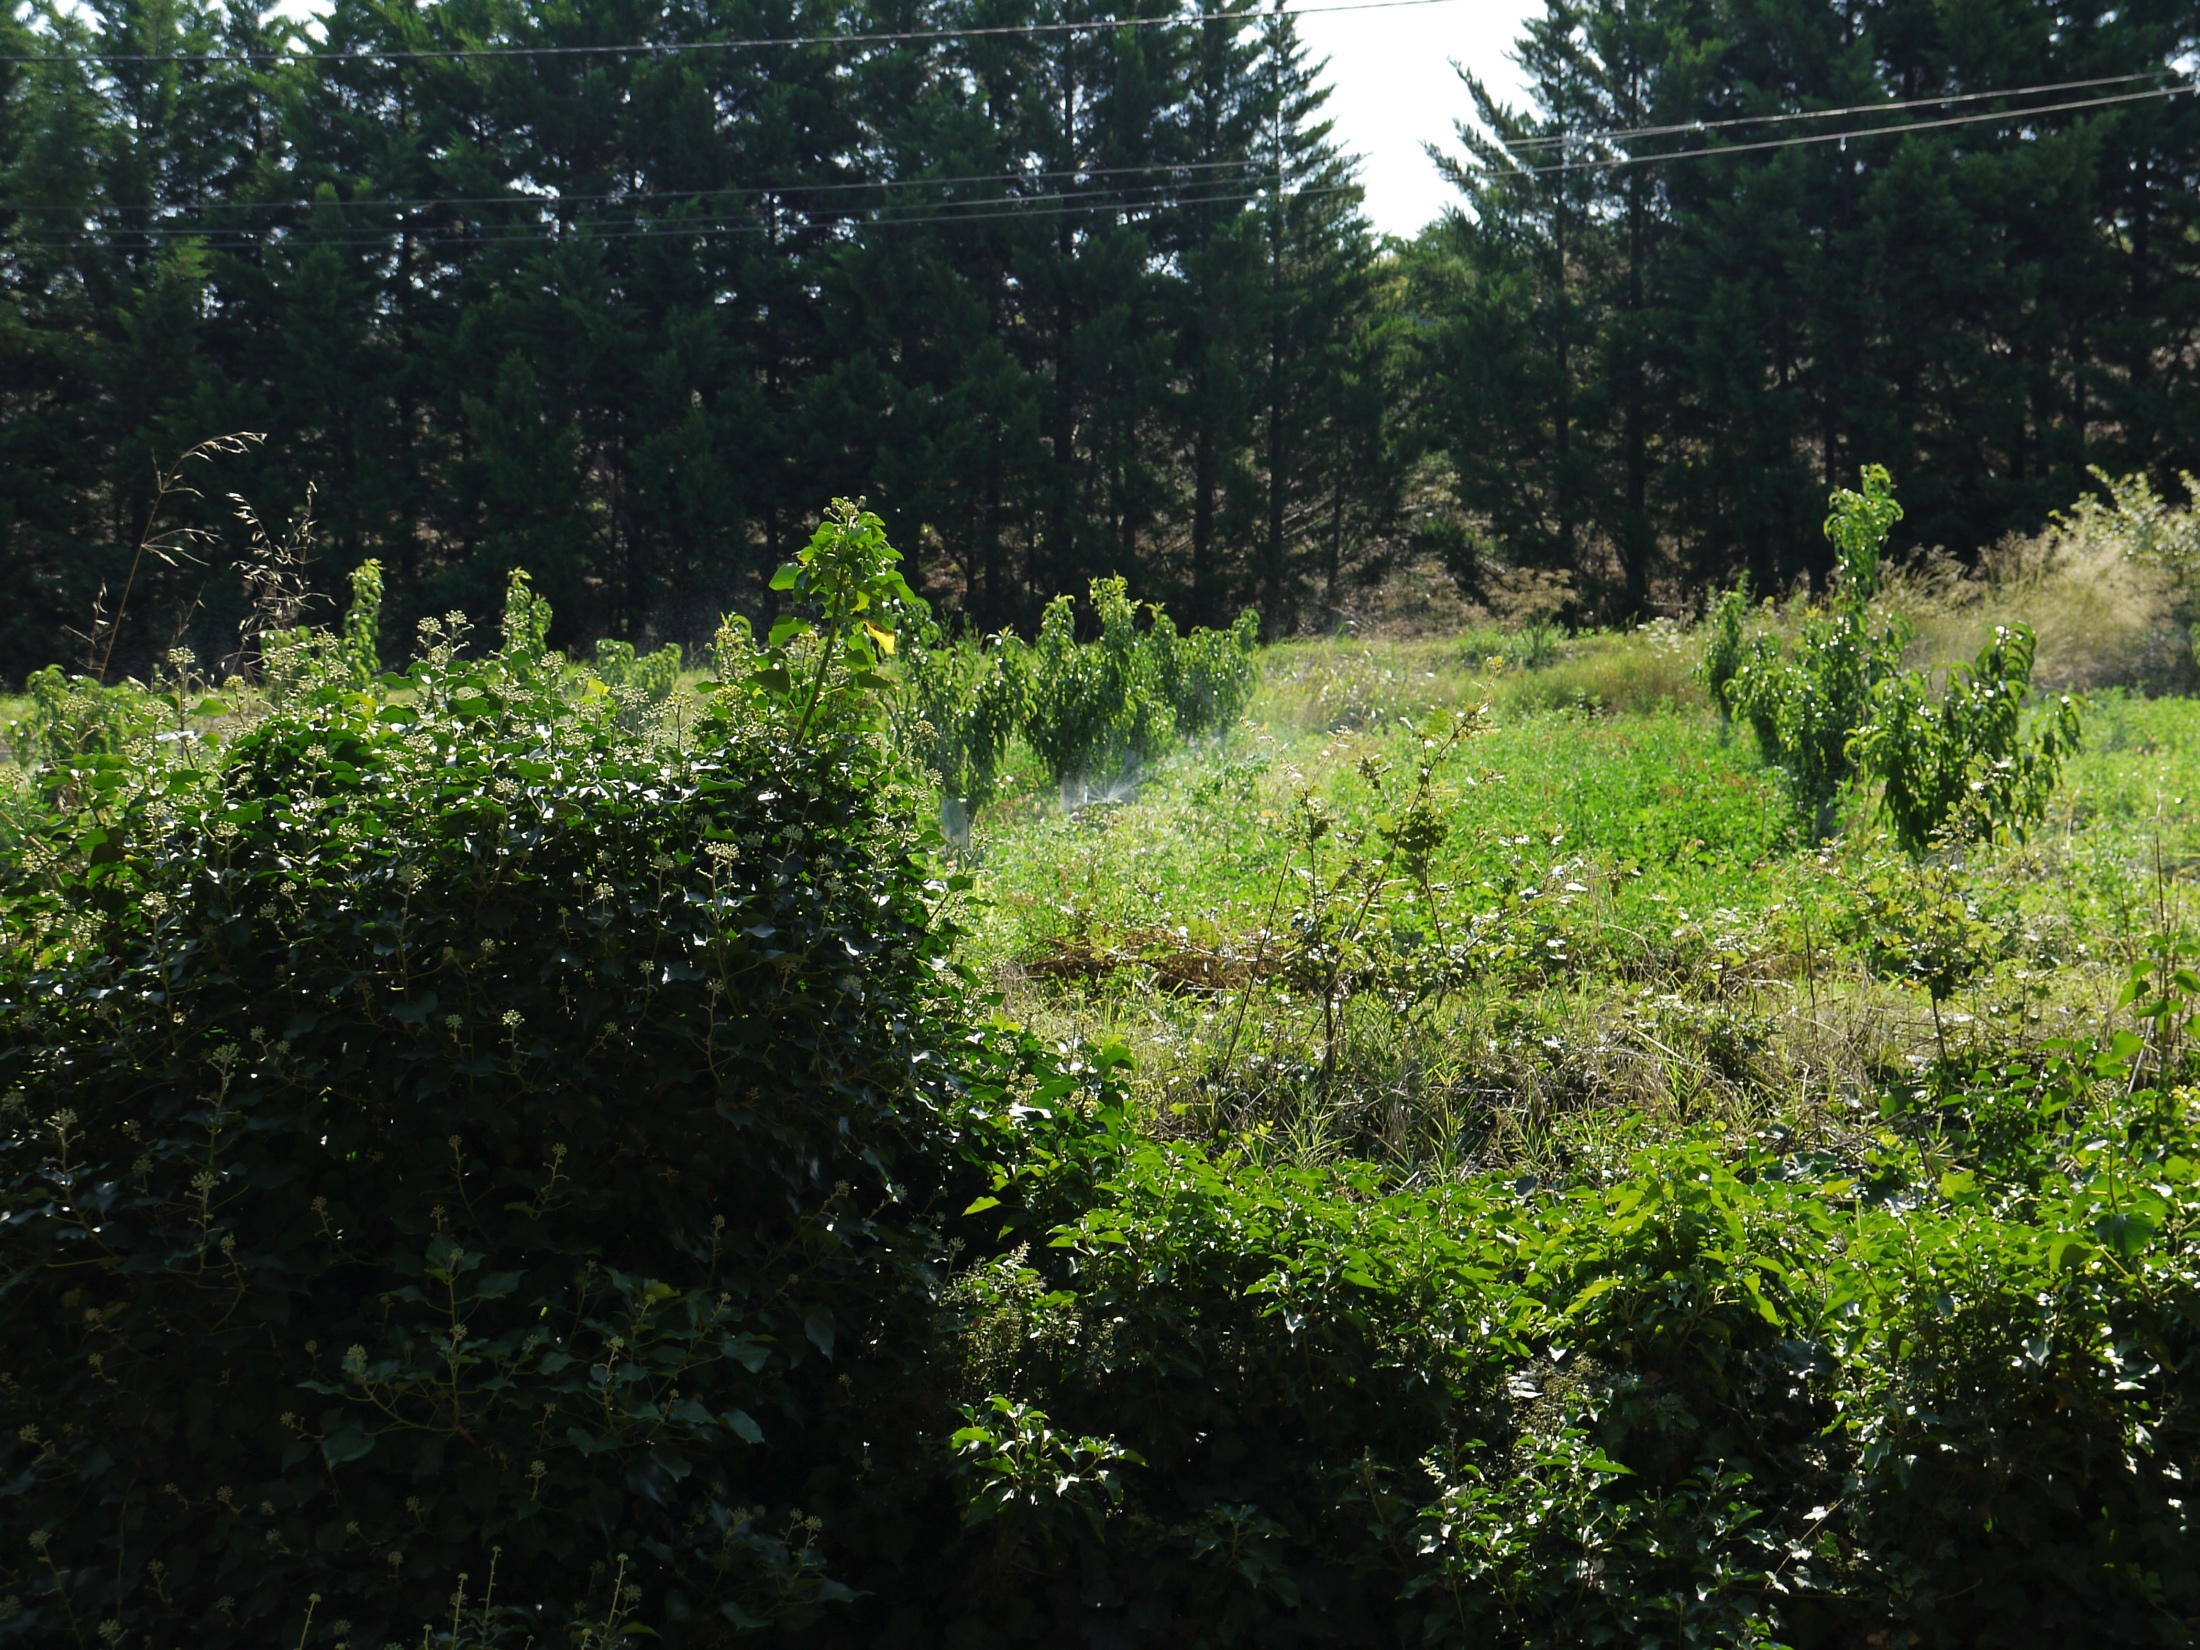
\includegraphics[width=\paperwidth]{img/annexe_irrigation}}%
\begin{frame}
  \vspace{-1em}  
  \begin{minipage}[t][.8\textheight]{\textwidth}
    \color{\cnGrey}{\LARGE{~}}

    \vfill

  \hfill \small{Photo credit : James Linton}
  \end{minipage}
  
\end{frame}
}

%-=-=-=-=-=-=-=-=-=-=-=-=-=-=-=-=-=-=-=-=-=-=-=-=
{
\usebackgroundtemplate{
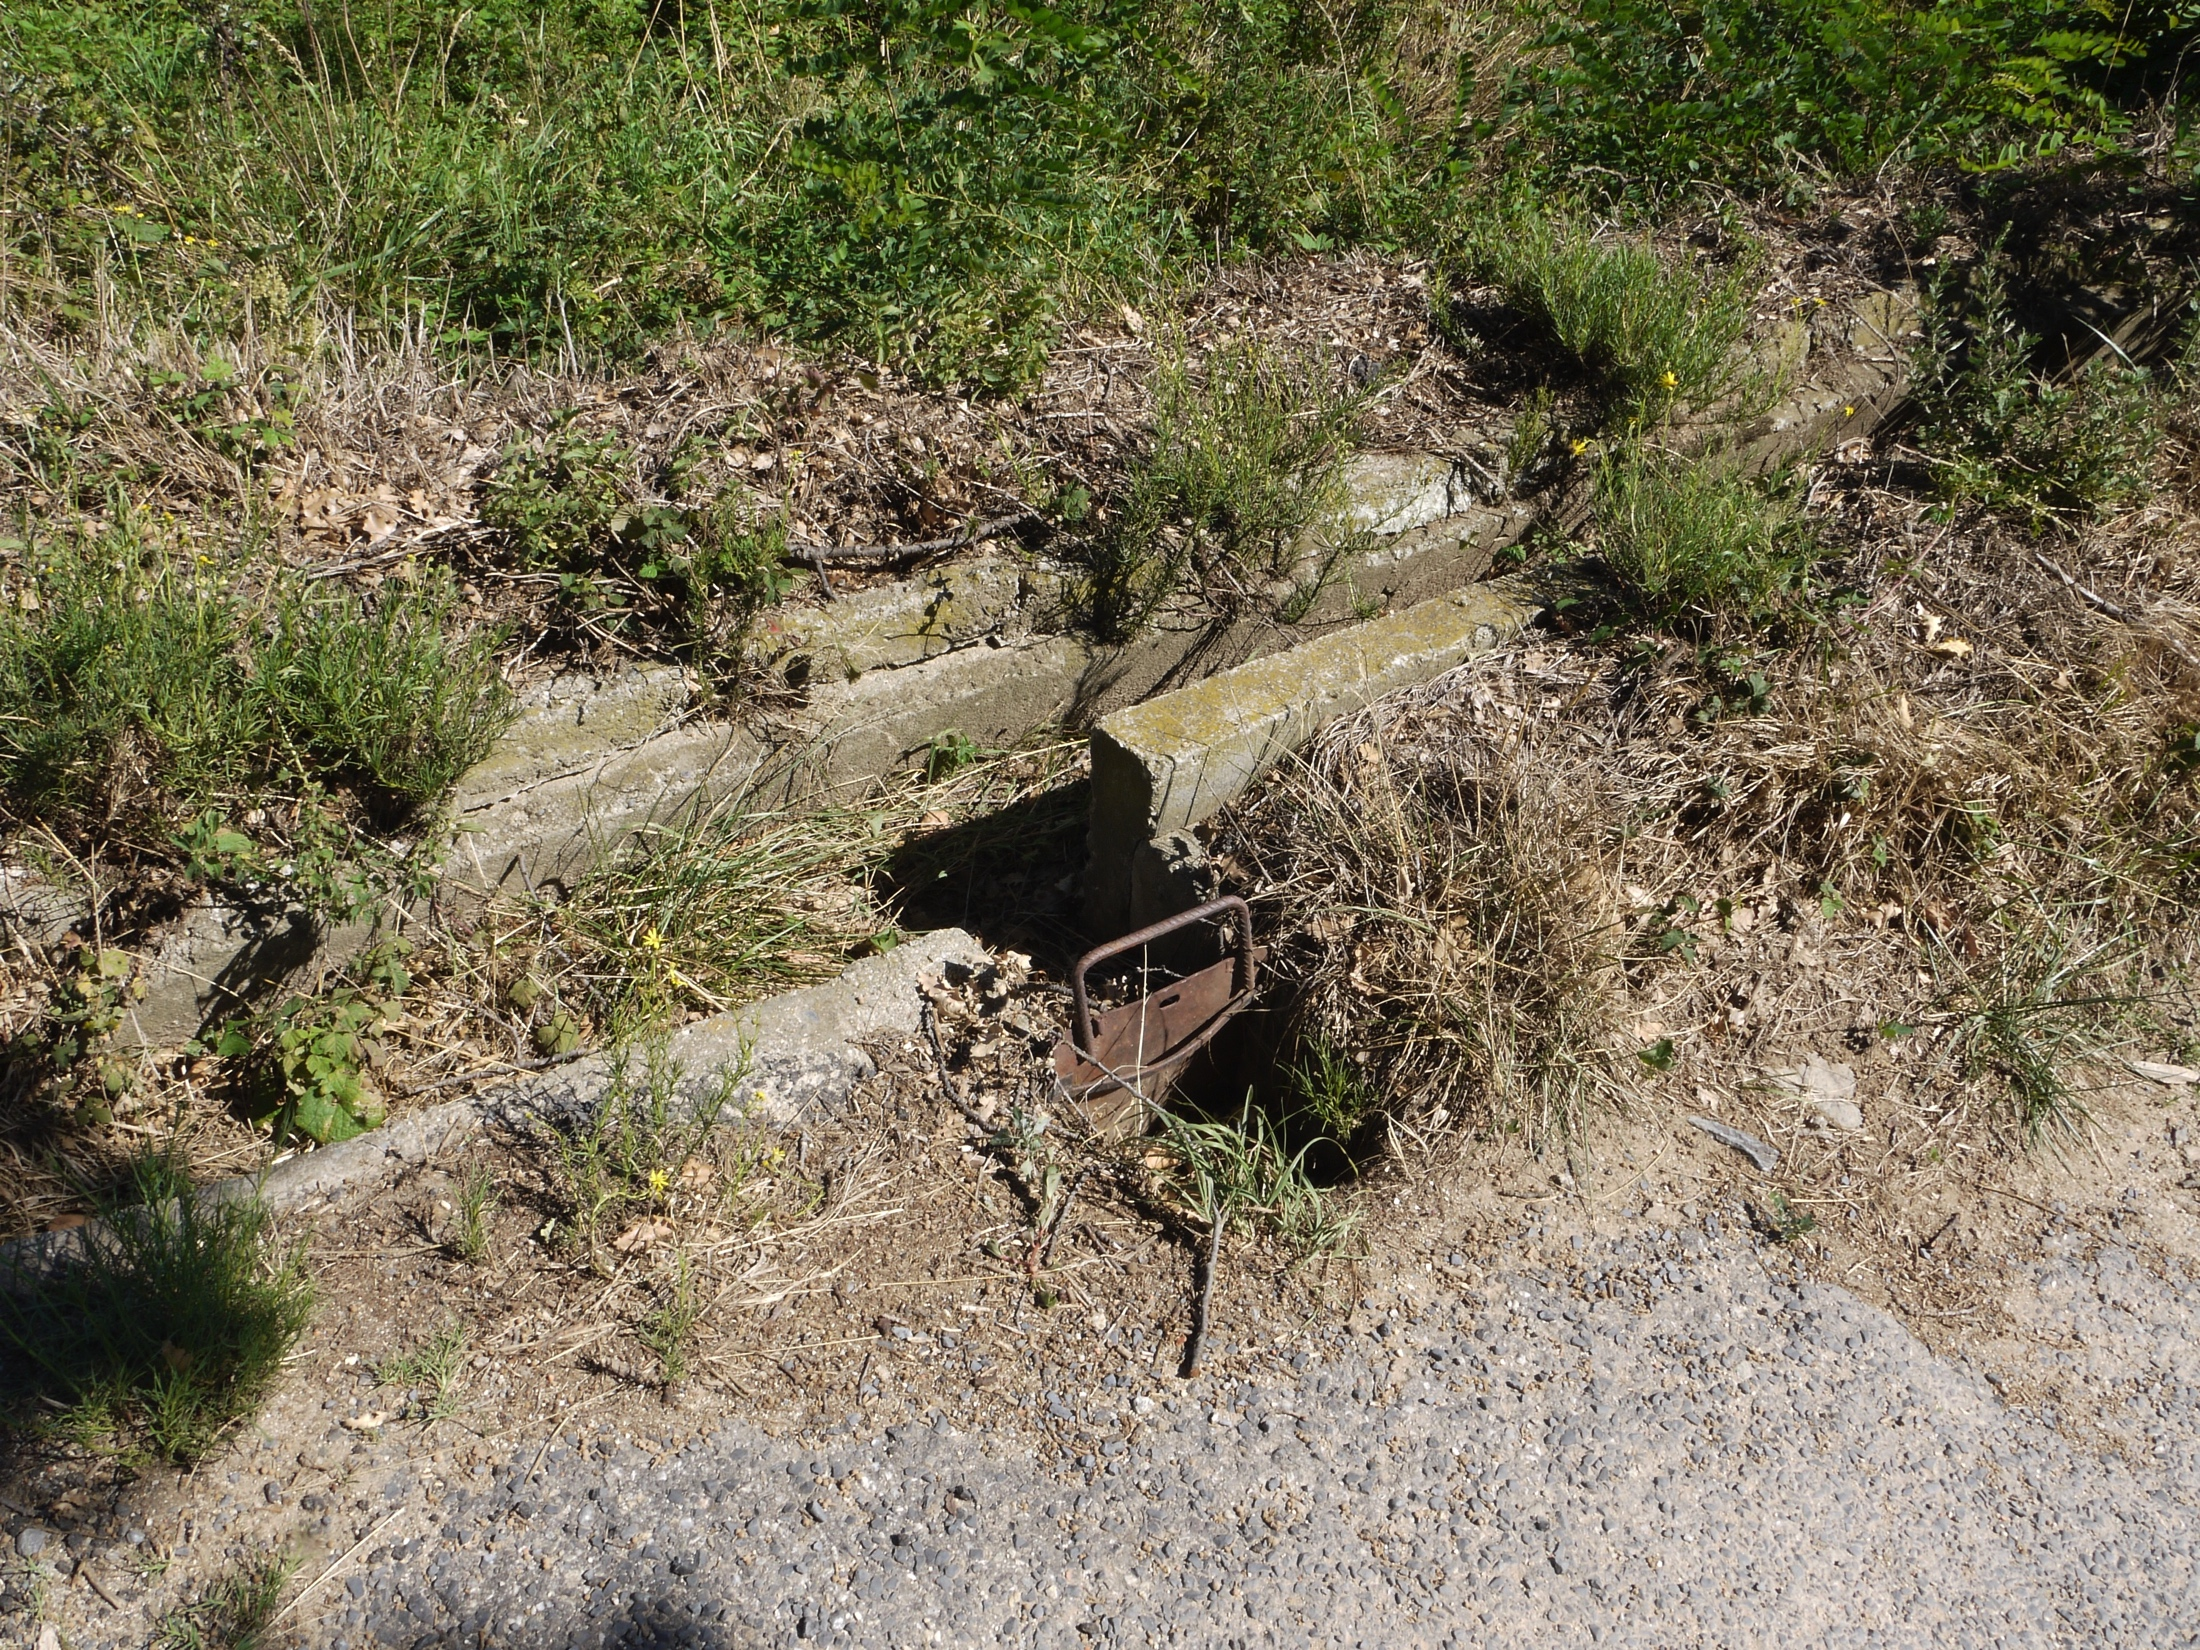
\includegraphics[width=\paperwidth]{img/annexe_old1}}%
\begin{frame}
  \vspace{-1em}  
  \begin{minipage}[t][.8\textheight]{\textwidth}
    \color{\cnGrey}{\LARGE{~}}

    \vfill

  \hfill \small{Photo credit : James Linton}
  \end{minipage}
  
\end{frame}
}

%-=-=-=-=-=-=-=-=-=-=-=-=-=-=-=-=-=-=-=-=-=-=-=-=
{
\usebackgroundtemplate{
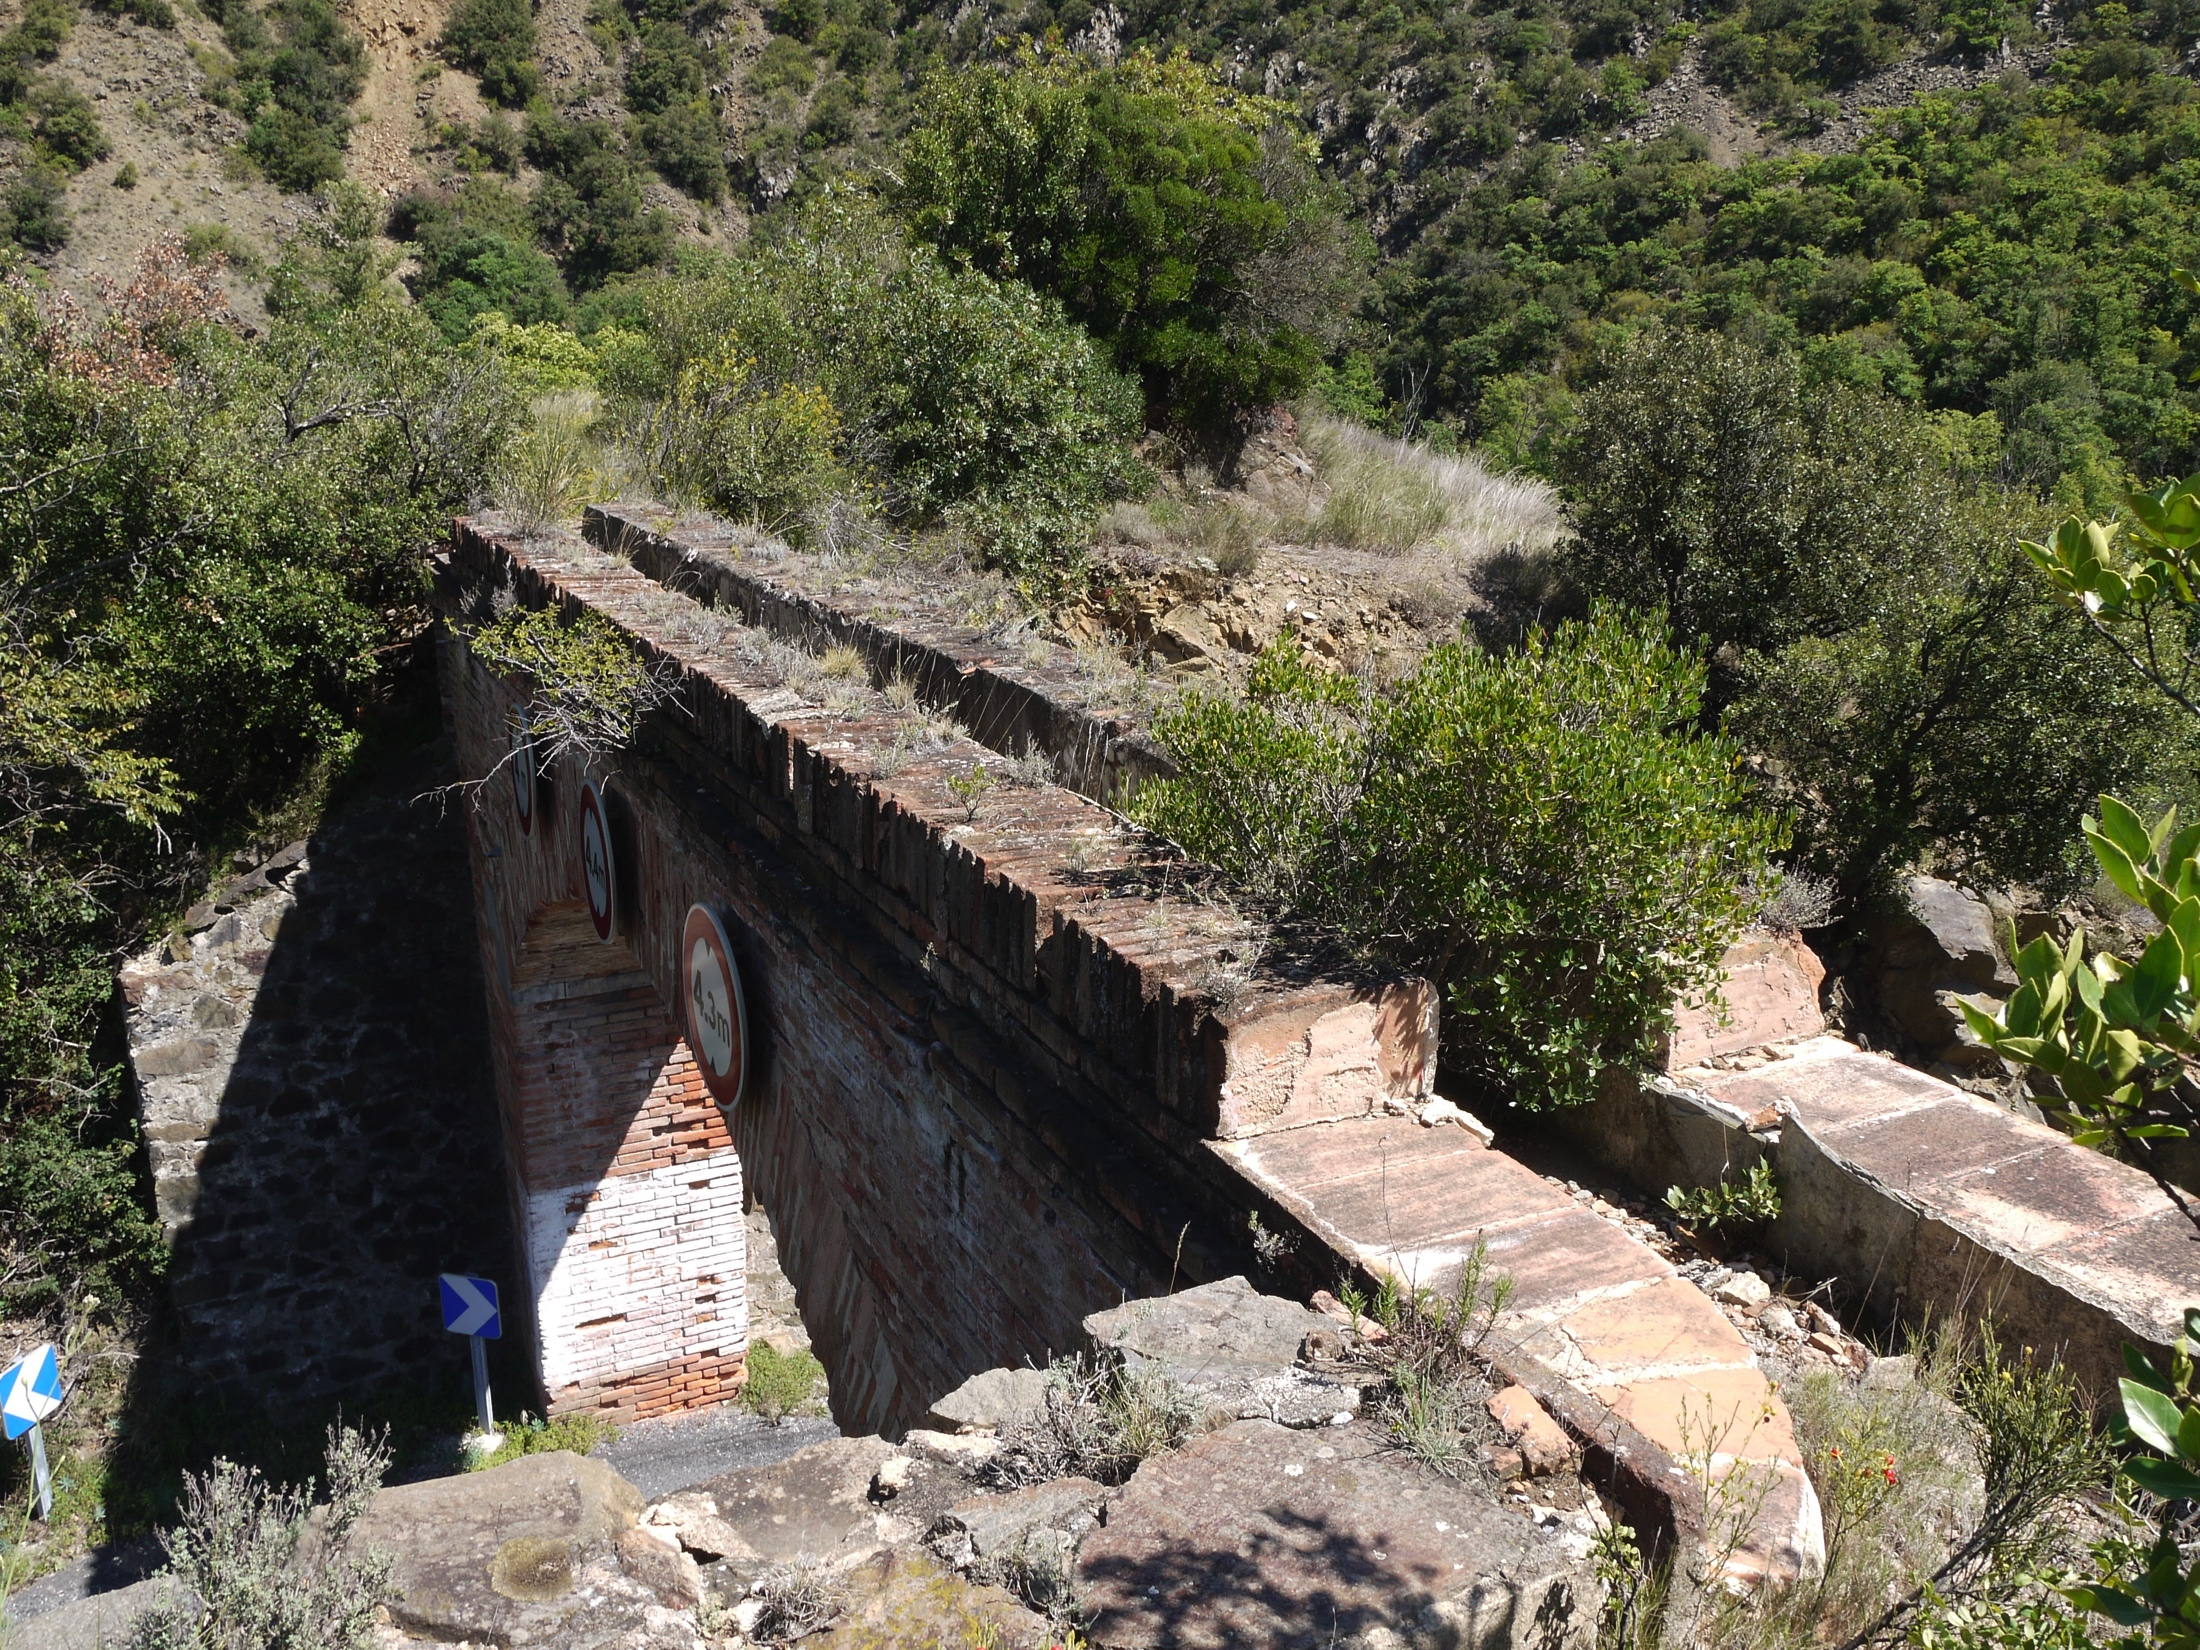
\includegraphics[width=\paperwidth]{img/annexe_old2}}%
\begin{frame}
  \vspace{-1em}  
  \begin{minipage}[t][.8\textheight]{\textwidth}
    \color{\cnGrey}{\LARGE{~}}

    \vfill

  \hfill \small{Photo credit : James Linton}
  \end{minipage}
  
\end{frame}
}

%-=-=-=-=-=-=-=-=-=-=-=-=-=-=-=-=-=-=-=-=-=-=-=-=
{
\usebackgroundtemplate{
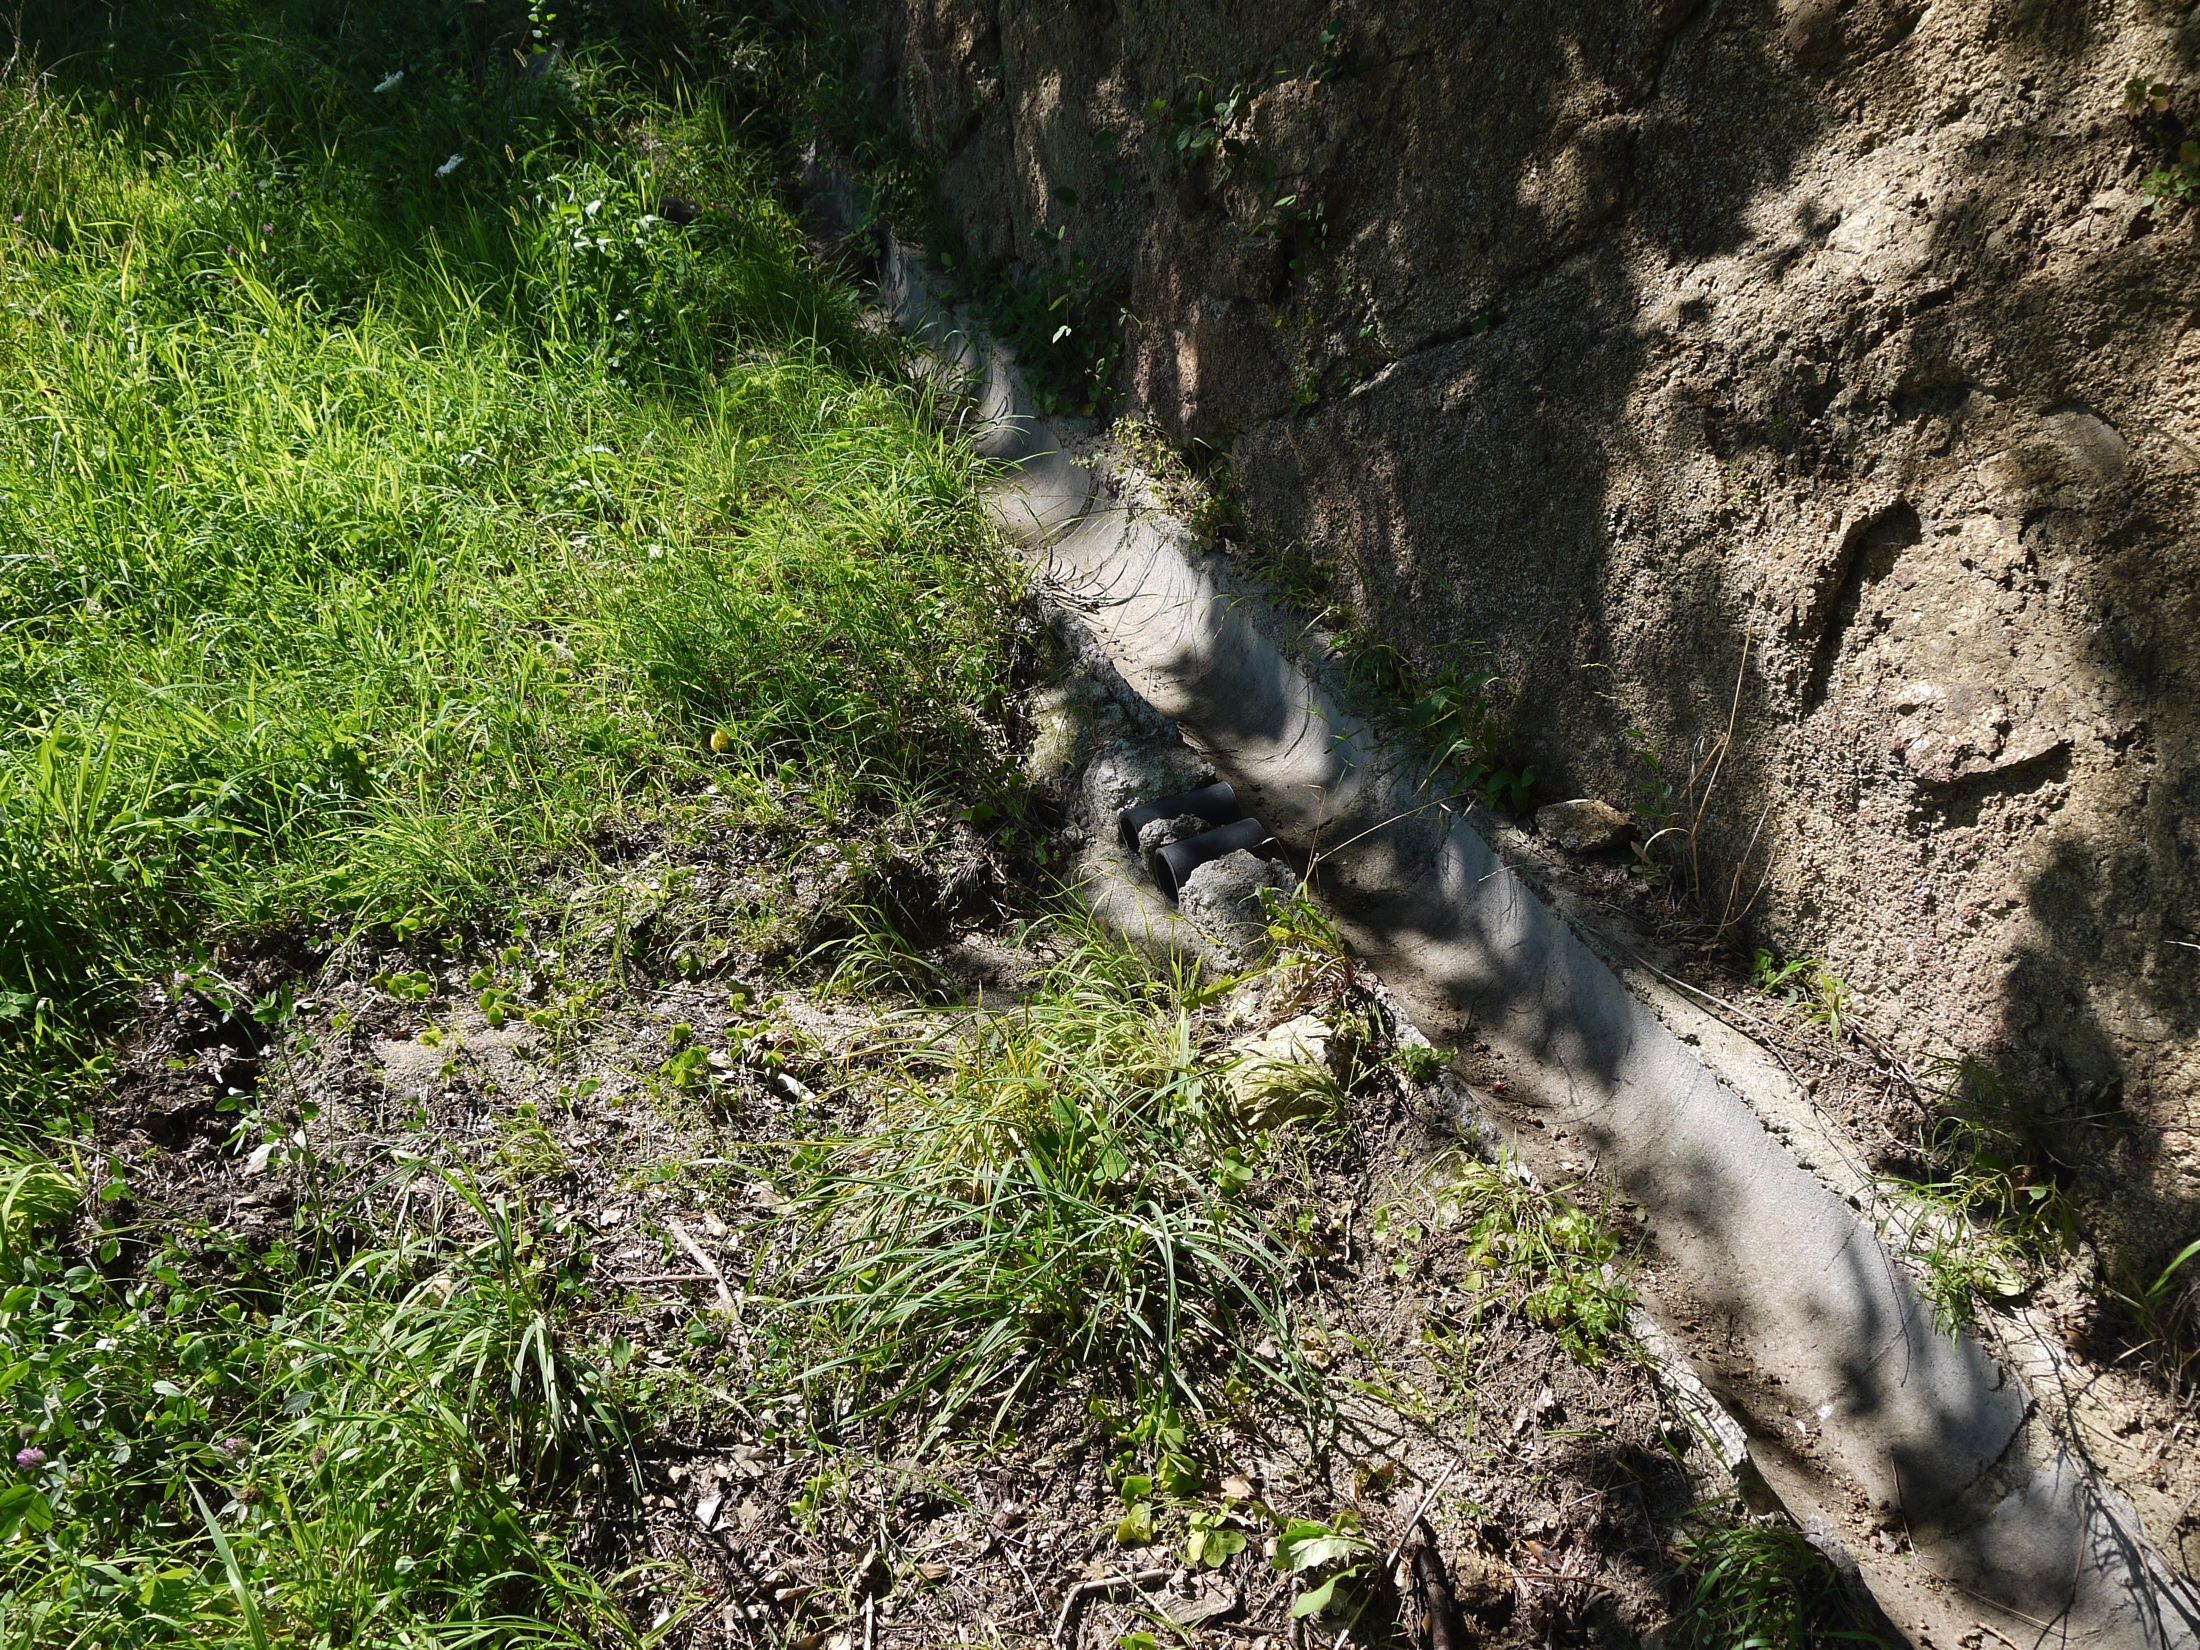
\includegraphics[width=\paperwidth]{img/annexe_rai}}%
\begin{frame}
  \vspace{-1em}  
  \begin{minipage}[t][.8\textheight]{\textwidth}
    \color{\cnGrey}{\LARGE{~}}

    \vfill

  \hfill \small{Photo credit : James Linton}
  \end{minipage}
  
\end{frame}
}

%-=-=-=-=-=-=-=-=-=-=-=-=-=-=-=-=-=-=-=-=-=-=-=-=
{
\usebackgroundtemplate{
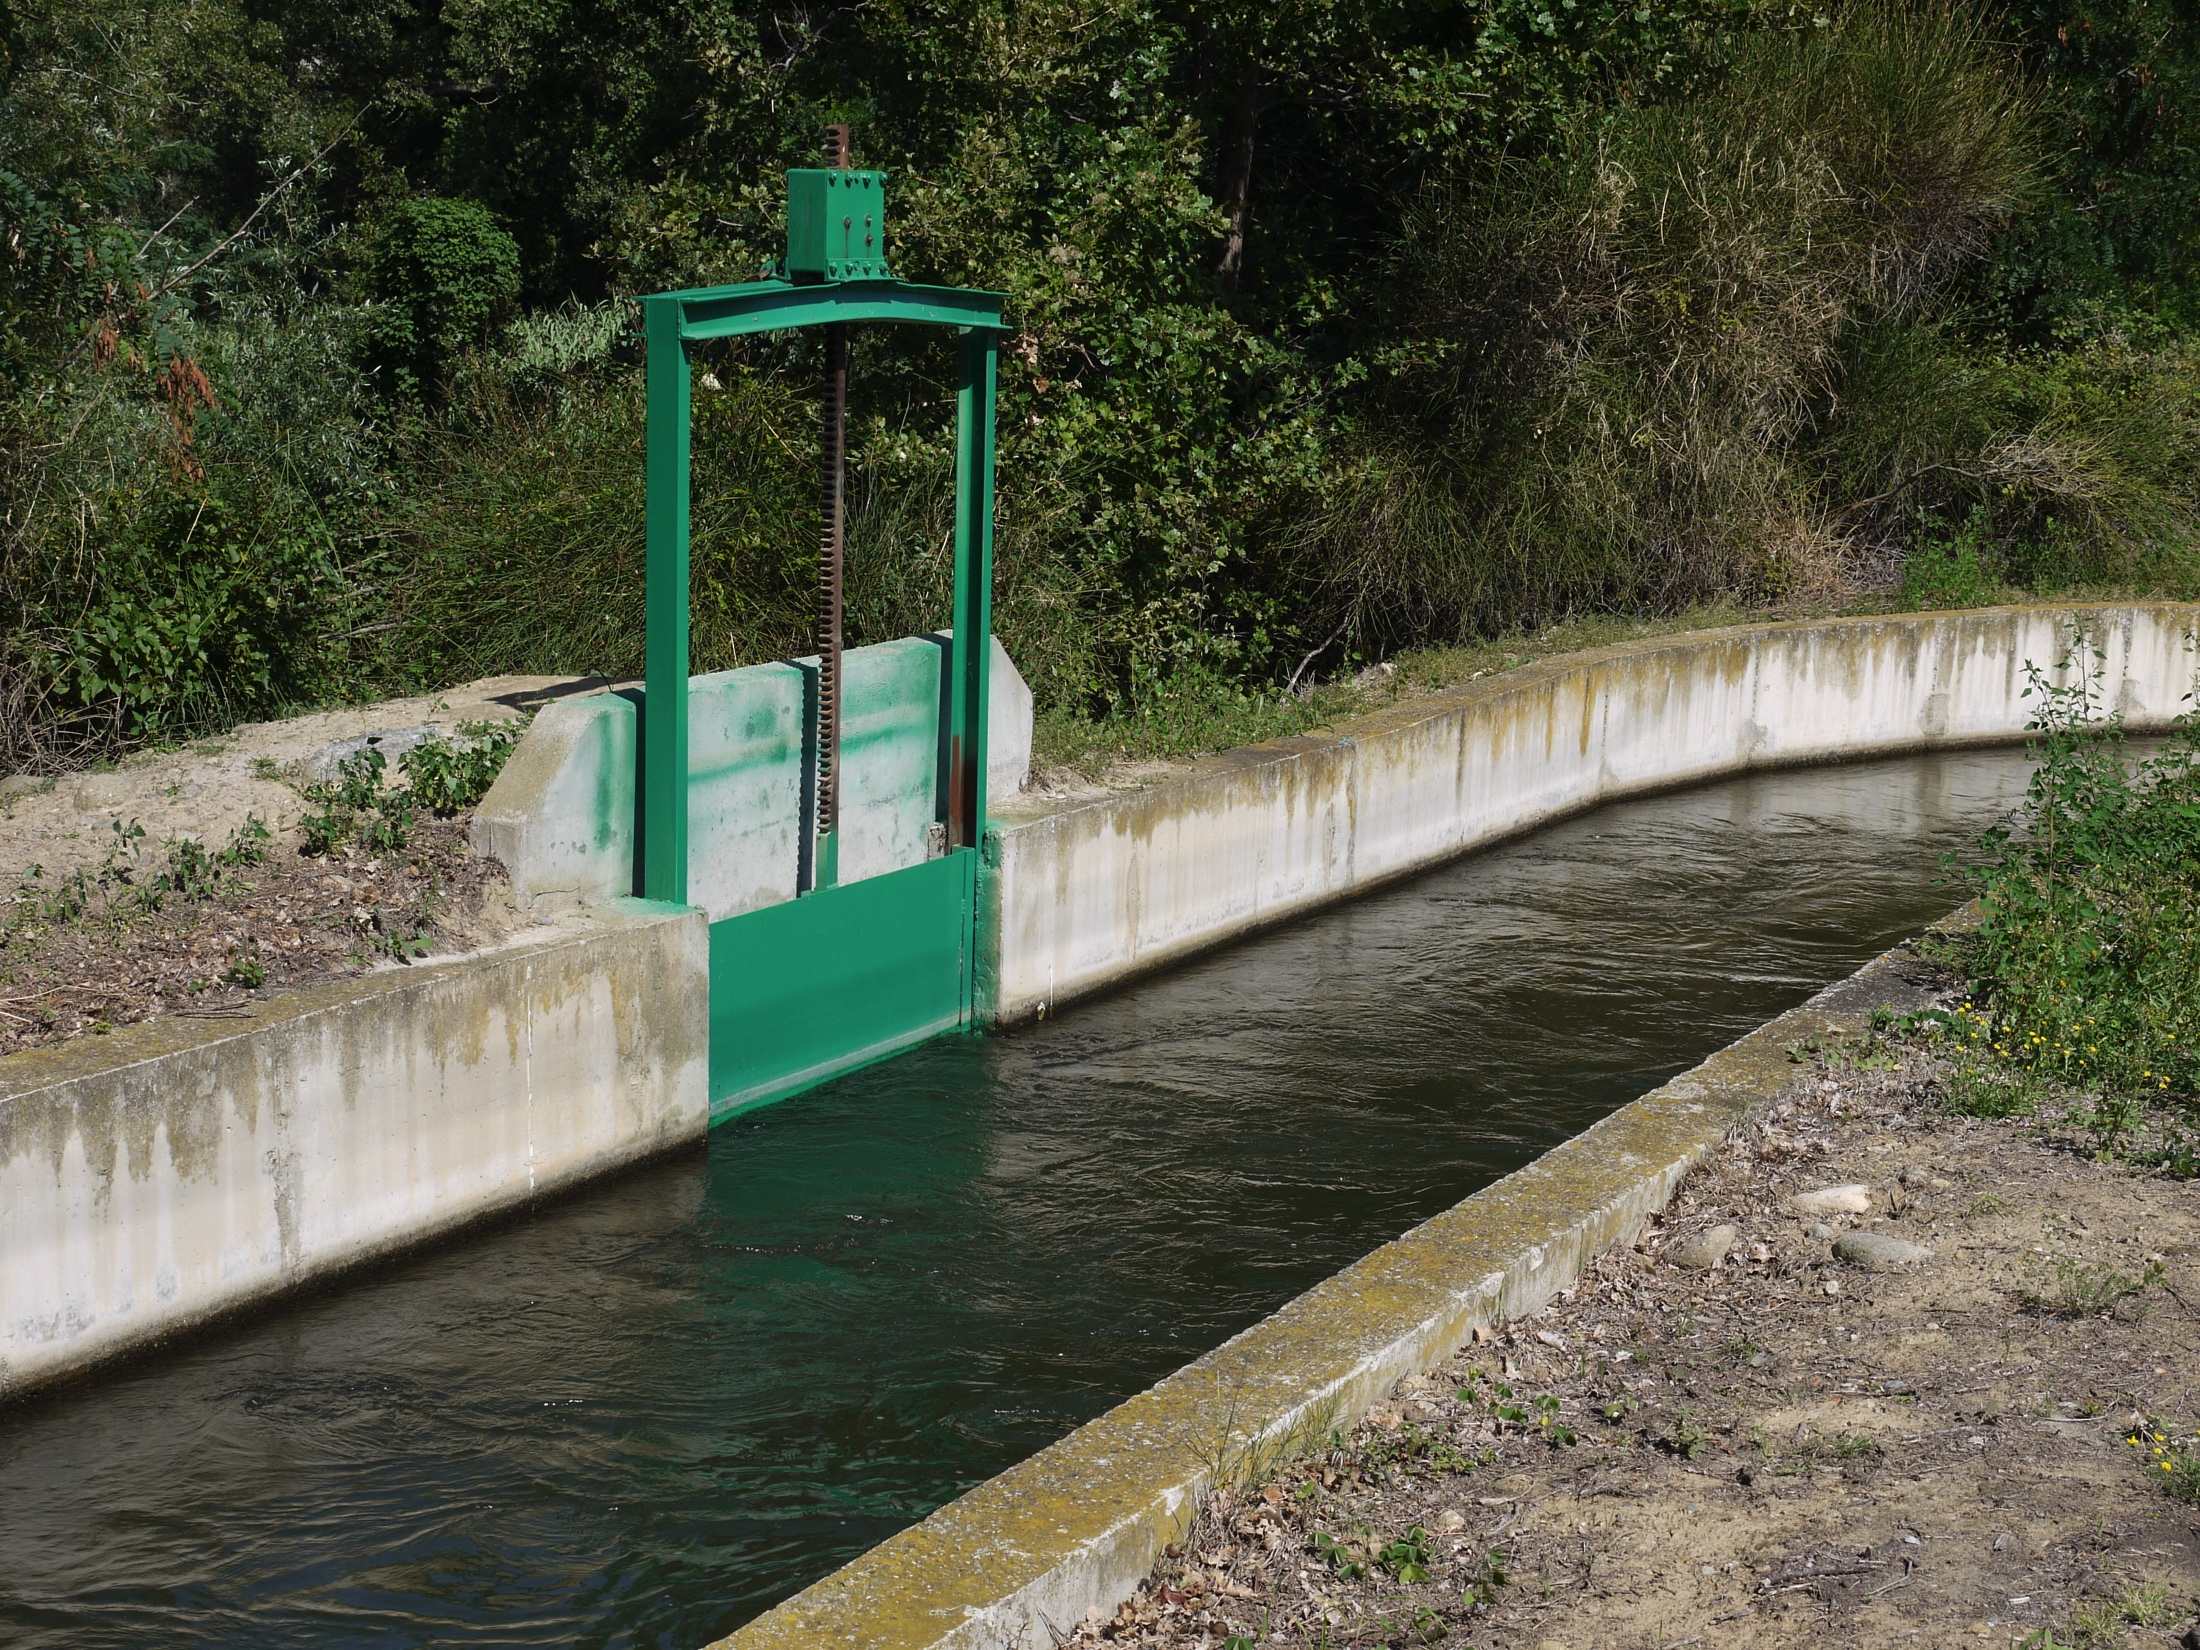
\includegraphics[width=\paperwidth]{img/annexe_vanne}}%
\begin{frame}
  \vspace{-1em}  
  \begin{minipage}[t][.8\textheight]{\textwidth}
    \color{\cnGrey}{\LARGE{~}}

    \vfill

  \hfill \small{Photo credit : James Linton}
  \end{minipage}
  
\end{frame}
}

%-=-=-=-=-=-=-=-=-=-=-=-=-=-=-=-=-=-=-=-=-=-=-=-=
{
\usebackgroundtemplate{
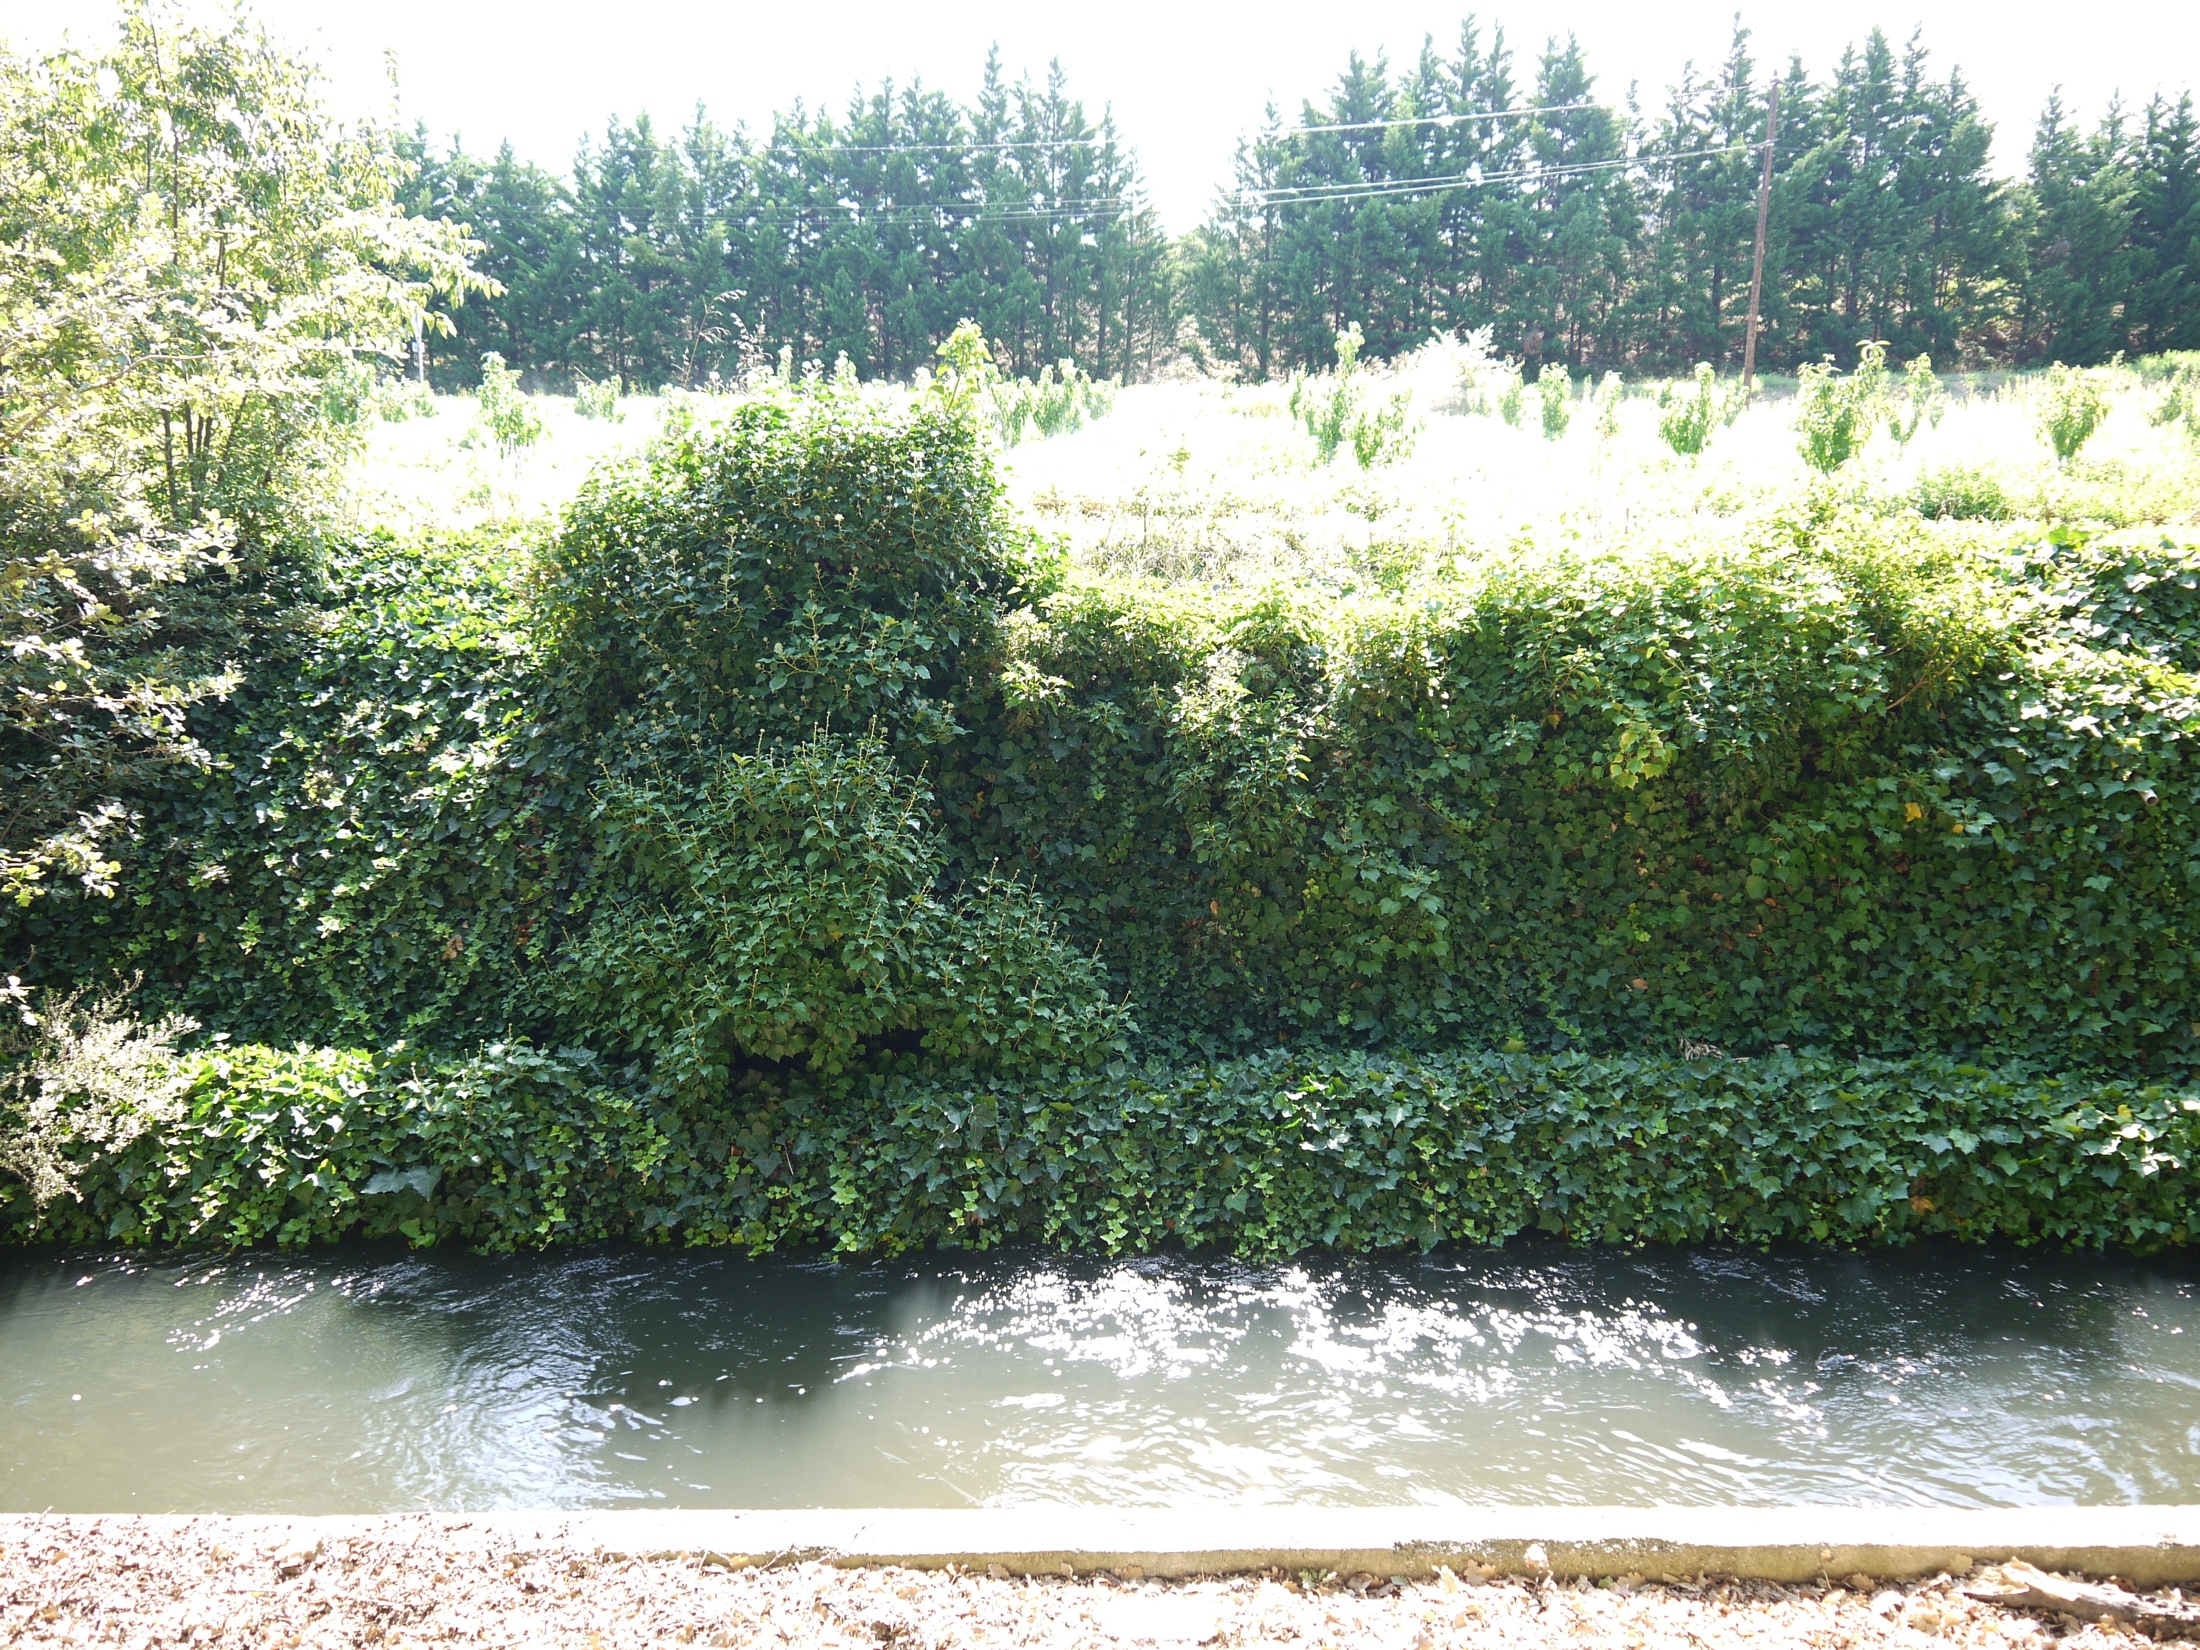
\includegraphics[width=\paperwidth]{img/annexe_verger}}%
\begin{frame}
  \vspace{-1em}  
  \begin{minipage}[t][.8\textheight]{\textwidth}
    \color{\cnGrey}{\LARGE{~}}

    \vfill

  \hfill \small{Photo credit : James Linton}
  \end{minipage}
  
\end{frame}
}


%-=-=-=-=-=-=-=-=-=-=-=-=-=-=-=-=-=-=-=-=-=-=-=-=
%	FRAME: LOACL VISION
%-=-=-=-=-=-=-=-=-=-=-=-=-=-=-=-=-=-=-=-=-=-=-=-=
%
%\begin{frame}[c]{What about Wittfogel ?}
%\begin{alertblock}{\textsc{Note}}
%	\begin{itemize}
%		\item We can consider local politicians as Leon Jean Grégory as the heirs of the hydraulic elite. They try to improve their own vision of modernity. 
%		\item Leon Jean Grégory is still in memory and his legacy is maintained by the ASA. Indeed today, this vision is a way to oppose irritants to the water agency. 
%		\item underlines the shift from a policy of demand to supply policy
%	\end{itemize}
%\end{alertblock}
%\end{frame}
%
%%-=-=-=-=-=-=-=-=-=-=-=-=-=-=-=-=-=-=-=-=-=-=-=-=
%%	FRAME: LOACL VISION
%%-=-=-=-=-=-=-=-=-=-=-=-=-=-=-=-=-=-=-=-=-=-=-=-=
%
%\begin{frame}[c]{What about Wittfogel ?}
%\begin{alertblock}{\textsc{Note}}
%	\begin{itemize}
%		\item We can consider local politicians as Leon Jean Grégory as the heirs of the hydraulic elite. They try to improve their own vision of modernity. 
%		\item Leon Jean Grégory is still in memory and his legacy is maintained by the ASA. Indeed today, this vision is a way to oppose irritants to the water agency. 
%		\item underlines the shift from a policy of demand to supply policy
%	\end{itemize}
%\end{alertblock}
%\end{frame}
%
%%-=-=-=-=-=-=-=-=-=-=-=-=-=-=-=-=-=-=-=-=-=-=-=-=
%%	FRAME: Simplicity in complexity
%%-=-=-=-=-=-=-=-=-=-=-=-=-=-=-=-=-=-=-=-=-=-=-=-=
%%\section{Simplicity in complexity}
%\section{Death by certainty}
%
%%-=-=-=-=-=-=-=-=-=-=-=-=-=-=-=-=-=-=-=-=-=-=-=-=
%%	FRAME: CHANGES 
%%-=-=-=-=-=-=-=-=-=-=-=-=-=-=-=-=-=-=-=-=-=-=-=-=
%\begin{frame}[c]{Change in perspective}
%however, a more complex set of dialectical relations is at play in this situation, requiring a subtler explanatory tool.
%	\begin{block}{\textsc{hypotheses}}
%	\begin{itemize}
%		\item We show that the dam has had the effect of transferring expertise and social power from local to central authority, but not in a direct way.
%		\item Rather, the production of hydrological certainty in the form of assured and regular flows has weakened the local social structures and relations that had evolved to accommodate - and were sustained by - hydrological uncertainty and periodical scarcity
%	\end{itemize}
%	\end{block}
%\end{frame}
%
%%-=-=-=-=-=-=-=-=-=-=-=-=-=-=-=-=-=-=-=-=-=-=-=-=
%%	FRAME: Technological Changes 
%%-=-=-=-=-=-=-=-=-=-=-=-=-=-=-=-=-=-=-=-=-=-=-=-=
%\begin{frame}[c]{Technological Changes}
%	\begin{block}{\textsc{Facts}}
%		dam is filling its two main tasks : irrigation and reducing flood peaks
%	\end{block}
%	\begin{itemize}
%		\item shift of gravity irrigation to pressurized irrigation
%		\item gravity irrigation : 
%			\begin{itemize}
%				\item role of socio-spatial entropy reduction
%			\end{itemize}
%		\item pressurized irrigation
%			\begin{itemize}
%				\item expand irrigated areas (at constant volume)
%				\item regroup plots more easily
%				\item reduce the arduous nature of irrigation (automatization)
%			\end{itemize}
%	\end{itemize}
%\end{frame}
%
%%-=-=-=-=-=-=-=-=-=-=-=-=-=-=-=-=-=-=-=-=-=-=-=-=
%%	FRAME: what have we to lost
%%-=-=-=-=-=-=-=-=-=-=-=-=-=-=-=-=-=-=-=-=-=-=-=-=
%\begin{frame}[c]{What have we lost}
%	\begin{itemize}
%		\item It provokes a vertical shift of responsibility
%		\begin{itemize}
%			\item historical responsibility was linked to the neighbors
%			\item today is being linked to ASA administrators
%		\end{itemize}
%		\item Canals had a responsibility the recharging of aquifers, it question the Leon Jean Grégory legacy.
%	\end{itemize}
%\end{frame}

%-=-=-=-=-=-=-=-=-=-=-=-=-=-=-=-=-=-=-=-=-=-=-=-=
%	FRAME: The hydrosocial cycle
%-=-=-=-=-=-=-=-=-=-=-=-=-=-=-=-=-=-=-=-=-=-=-=-=
\begin{frame}[c]{The hydro social cycle}
	\vspace{-2em}
	We employ the concept of the hydro social cycle  - which borrows from Wittfogel's dialectic, but demands a more complex account of hydro social relations -- to explain these developments.
	\begin{figure}
	\vspace{-1em}
	\centering
	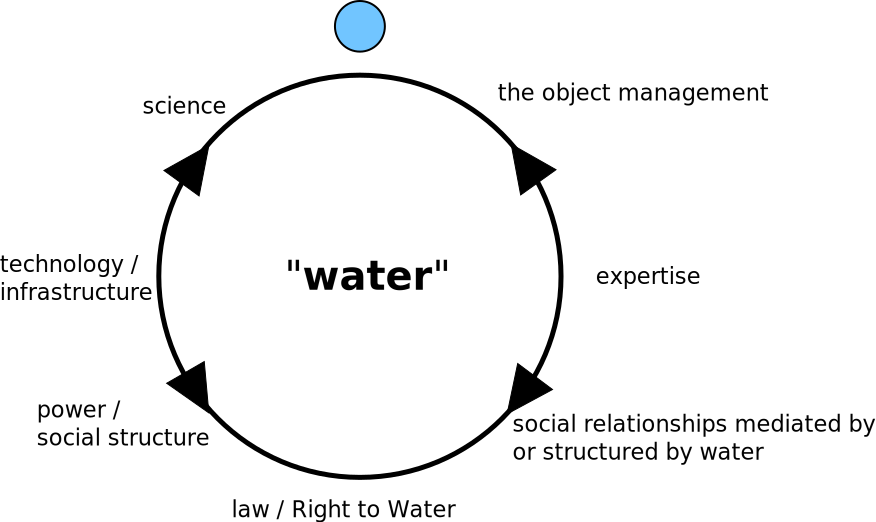
\includegraphics[width = 0.8\textwidth]{img/hydrosocial_cycle}
	 \caption{hydrosocial cycle}
\end{figure}
	
\end{frame}

%%-=-=-=-=-=-=-=-=-=-=-=-=-=-=-=-=-=-=-=-=-=-=-=-=
%%
%%	SECTION: CONCLUSION
%%
%%-=-=-=-=-=-=-=-=-=-=-=-=-=-=-=-=-=-=-=-=-=-=-=-=
%\section*{Conclusion}
%
%%-=-=-=-=-=-=-=-=-=-=-=-=-=-=-=-=-=-=-=-=-=-=-=-=
%%	FRAME:
%%-=-=-=-=-=-=-=-=-=-=-=-=-=-=-=-=-=-=-=-=-=-=-=-=
%
%\begin{frame}[c]{Conclusion}
%\vspace{-2em}
%\begin{exampleblock}{Our hypothesizing}
%	Some of the longer-term consequences of the dam in terms of its unintended impacts on the agricultural sector of the region and, ultimately, on the influence of the state.
%\end{exampleblock}
%
%\end{frame}


\end{document}


